%\documentclass[runningheads]{llncs}

\documentclass{article}
\usepackage{nips_2018}


%\usepackage[cmex10]{amsmath, mathtools}
\usepackage{amsmath}
%\usepackage[fleqn]{amsmath}
%\usepackage{amssymb,amsbsy,amsfonts,amsthm}
\usepackage{amssymb,amsbsy,amsfonts}
\usepackage{bm}
\usepackage{enumerate}
\usepackage{url}
\usepackage[ruled,vlined]{algorithm2e}
\usepackage{fancyvrb}
\usepackage{yfonts}
\usepackage{multirow}
\usepackage{multicol}
\usepackage{adjustbox}
%\usepackage[margin=6.5em]{geometry}
\usepackage{makecell} % thicker table separator
\usepackage{booktabs}


\usepackage{subfigure}
\usepackage{wrapfig}
\usepackage{tikz}
%\input{../tikz.conf}

\usetikzlibrary{bayesnet}

%%%%%%%%%%% Box 
\usepackage{calc}%    For the \widthof macro
\usepackage{xparse}%  For \NewDocumentCommand
\newcommand{\tikzmark}[1]{\tikz[overlay,remember picture] \node (#1) {};}


%\input{./header.tex}
%%%%%%%%%% Math
\renewcommand{\text}{\textnormal}
%\newcommand{\pr}{\mathbf{p}}
\newcommand{\pr}{p}
\newcommand{\p}{p}
\newcommand{\E}{\mathbb{E}}
\newcommand{\divkk}{\mathbb{K}}
\newcommand{\entropy}{\mathbb{H}}
\newcommand{\gem}{\mathrm{GEM}}
\newcommand{\Mult}{\mathrm{Mult}}
\newcommand{\DP}{\mathrm{DP}}
\newcommand{\IBP}{\mathrm{IBP}}
\newcommand{\M}{\mathcal{M}}
\newcommand{\V}{\mathcal{V}}
\newcommand{\N}{\mathcal{N}}
\newcommand{\D}{\mathcal{D}}
\renewcommand{\L}{\mathcal{L}}
\newcommand{\mat}[1]{\mathbf{#1}}
\newcommand{\unit}{1\!\!1}
\newcommand{\zij}{z_{i\rightarrow j}}
\newcommand{\zji}{z_{i\leftarrow j}}
\newcommand{\Thetah}{\hat\Theta}
\newcommand{\Phih}{\hat\Phi}
\newcommand{\thetah}{\hat\theta}
\newcommand{\phih}{\hat\phi}

\newcommand\mms[1]{\vcenter{\hbox{$\scriptstyle #1$}}}

%\renewcommand{\Phi}{\mat{\Phi}}


%\date{avril 2015}

%\newtheorem{definition}{Definition}[section]
%\newtheorem{proposition}{Proposition}[section]
%\newtheorem{theorem}{Theorem}[section]
%\newtheorem{corollary}{Corollary}[section]
%\newtheorem{proof}{Proof}[section]


\begin{document}

\title{Supplementary material of \textit{Mixed-Membership Stochastic Block Models for Weighted Networks}}
	
\maketitle

%\begin{abstract}
%\end{abstract}

\section{Derivation of the collapsed variational updates}

The derivation of the collapsed variational updates is first obtained by maximizing the ELBO w.r.t $\gamma_{ijkk'}$ with:
%
\begin{align*}
\frac{\partial \L_Z}{\partial \gamma_{ijkk'}} &= \frac{\partial }{\partial \gamma_{ijkk'}}  \sum_{Z^{-ij}}\sum_{k_1=1}^K\sum_{k_2=1}^K  q(Z^{-ij}) \gamma_{ijk_1 k_2} (\log p(Y, Z^{-ij}, z_{i\rightarrow j}=k_1, z_{i\leftarrow j}=k_2|\Omega)+ \\
& \qquad \log q(Z^{-ij}, z_{i\rightarrow j}=k_1, z_{i\leftarrow j}=k_2) )   \\
&= E_{q(Z^{-ij})}[ p(Y, Z^{-ij}, z_{i\rightarrow j}=k, z_{i\leftarrow j}=k'|\Omega))] + H[Z^{-ij}] -\log(\gamma_{ijkk'}) +1
\end{align*}
%
By equating this derivative to zero, one obtains the following update:
\begin{equation} \label{eq1}
\gamma_{ijkk'} \propto \exp E_{q(Z^{-ij})} [\log P(z_{i\rightarrow j}=k, z_{i\leftarrow j}=k' | Y^{-ij}, Z^{-ij}, \Omega) ]
\end{equation}
%
with  $P(z_{i\rightarrow j}=k, z_{i\leftarrow j}=k' | Y^{-ij}, Z^{-ij}, \Omega)$ being the collapsed Gibbs update of WMMSB, of the form:
%
\begin{align*}
P(z_{i\rightarrow j}=k, z_{i\leftarrow j}=k' |Y^{-ij}, Z^{-ij}, \Omega) \propto (n_{\rightarrow ik}^{\Theta^{-j}} + \alpha_k) (n_{\leftarrow jk}^{\Theta^{-i}} + \alpha_{k'}) \mathrm{NB}\left(y_{ij}; n^{Y^{-ij}}_{kk'} + r, \frac{p}{p\,n^{\Phi^{-ij}}_{\bm{.}kk'} + 1} \right)
\end{align*}
%
with count statistics given by the following equations:

%\begin{align} \label{eq:sss}
%    n^{\Theta}_{\rightarrow ik} &= \sum_{j, k'} \gamma_{ijkk'}        & n^{\Theta}_{\leftarrow jk'} &= \sum_{i, k} \gamma_{ijkk'}  \nonumber \\
%    n^{\Phi}_{xkk'} &= \sum_{ij:y_{ij}=x} \gamma_{ijkk'}  & n^{Y}_{kk'} &= \sum_{ij} y_{ij}\gamma_{ijkk'}
%\end{align}

\begin{align*}                                                                                                                                        
&n^{\Theta}_{\rightarrow ik} = \sum_j \delta(\zij=k)\\
&n^{Y}_{kk'} = \sum_{ij} y_{ij}\delta(\zij=k, \zji=k') \\
&n^{\Phi}_{\bm{.}kk'} = \sum_{ij} \delta( \zij=k, \zji=k') 
\end{align*}   

By applying a first order Taylor expansion on Eq.~\eqref{eq1}, following \cite{teh2007collapsed}, one obtains:

\begin{equation}
\gamma_{ijkk'} \propto (E_{q(Z^{-ij})}[n_{\rightarrow ik}^{\Theta^{-j}}] + \alpha_k) (E_{q(Z^{-ij})}[n_{\leftarrow jk}^{\Theta^{-i}}] + \alpha_{k'}) \mathrm{NB}\left(y_{ij}; E_{q(Z^{-ij})}[n^{Y^{-ij}}_{kk'}] + r, \frac{p}{p\,E_{q(Z^{-ij})}[n^{\Phi^{-ij}}_{\bm{.}kk'}] + 1} \right) \nonumber
\end{equation}

Finally, using a Gaussian approximation (as in \textit{e.g.} \cite{asuncion2009smoothing}), one can estimate the expectations $E_{q(Z^{-ij})}[n_{\rightarrow ik}^{\Theta^{-j}}], E_{q(Z^{-ij})}[n_{\leftarrow jk}^{\Theta^{-i}}]$ and  $E_{q(Z^{-ij})}[n^{\Phi^{-ij}}_{\bm{.}kk'}]$ with the counts defined in Eq. 2 of Section 3.1.

\section{Beta-Gamma updates}

In the WMMSB-bg model, the collapsed variational distribution takes the form:

\begin{equation*}
q(\Pi) = q(\Theta, \Phi|Z, R, P) q(Z)q(R)q(P)
\end{equation*}

The variational distribution for $r_{kk'}$ is taken in the Gamma family:  $q(r_{kk'}) = \textrm{Gamma}(a_{kk'},b_{kk'})$ for $1\leq k,k' \leq K$. The collapsed ELBO can thus be rewritten as:

\begin{align*}
\log p(Y) \geq \L_{Z,R,P} &= \E_{q}[\log p(Y, Z, R, P|\Omega)] + \textrm{H}[q(Z)] + \textrm{H}[q(R)] + \textrm{H}[q(P)] \\
                        &= \E_{q}[\log p(Y, Z)] + \textrm{H}[q(Z)] \\
                        &\qquad + \E_{q}[\log p(R|Y,Z,P)] + \textrm{H}[q(R)] \\
                        &\qquad +\E_{q}[\log p(P|Y,Z)] + \textrm{H}[q(P)] 
\end{align*}

\paragraph{Optimizing $\gamma_{ijkk'}$}

In the Beta-Gamma augmentation, the parameters $p$ and $r$ are marginalized in the update given by Eq.~\eqref{eq1}:
\begin{equation}
\gamma_{ijkk'} \propto \exp E_{q(Z^{-ij})} [\log E_{q(r_{kk'})}[E_{q(p_{kk'})}[ P(z_{i\rightarrow j}=k, z_{i\leftarrow j}=k' | Y^{-ij}, Z^{-ij}, \Omega) ] ] ] \nonumber
\end{equation}

By using a first order Taylor expansion, one obtains:

\begin{equation}
\gamma_{ijkk'} \propto (N_{\rightarrow ik}^{\Theta^{-j}} + \alpha_k) (N_{\leftarrow jk}^{\Theta^{-i}} + \alpha_{k'}) \mathrm{NB}\left(y_{ij}; N^{Y^{-ij}}_{kk'} + \E_{q}[r_{kk'}], \frac{\E_{q}[p_{kk'}]}{\E_{q}[p_{kk'}]\,N^{\Phi^{-ij}}_{\bm{.}kk'} + 1} \right) \nonumber
\end{equation}

\paragraph{Optimizing $r_{kk'}$}

We isolate the part of the ELBO than depends only on $r_{kk'}$ parameters ($a_{kk'}$ and $b_{kk'}$). Thus, we consider only the links that have been generated within the classes $k,k'$, denoted by $Y^{(kk')}$. Furthermore, as $y_{ij} \sim NB(r_{kk'}, p_{kk'})$ if $i$ is in class $k$ and $j$ in class $k'$, one has:

\begin{align*}
\L_{[r_{kk'}]} = \E_{q(r_{kk'})}[\log p(r_{kk'}|Y^{(kk')},Z^{(kk')},p_{kk'})] + \textrm{H}[q(r_{kk'})] \\
\end{align*}

By applying Bayes rules and dropping the normalizing term that does not depend on $r_{kk'}$, one gets:

\begin{align*}
\L_{[r_{kk'}]} &= \E_{q(r_{kk'})}[\log \left( p(Y^{(kk')}|Z^{(kk')}, r_{kk'}, p_{kk'}) p(r_{kk'}]) \right)] + \textrm{H}[q(r_{kk'})] \\
    &= \E_{q(r_{kk'})}[\log \left( \prod_{ij\in Y^{(kk')}} \dbinom{r_{kk'} + y_{ij}-1}{y_{ij}} (1-p_{kk'})^{r_{kk'}} p_k^{y_{ij}} p(r_{kk'}) \right) ] + \textrm{H}[q(r_{kk'})] \\
    &= \E_{q(r_{kk'})}[\log \left( (1-p_{kk'})^{r_{kk'} N^{\Phi}_{kk'}} p_{kk'}^{N^{Y}_{kk'}} p(r_{kk'}) \prod_{ij\in Y^{(kk')}} \frac{\Gamma(r_{kk'}+y_{ij})}{\Gamma(r_{kk'}) \Gamma(y_{ij}+1) }  \right) ] + \textrm{H}[q(r_{kk'})]
\end{align*}

If $y_{ij} = 0$, then $\frac{\Gamma(r_{kk'}+y_{ij})}{\Gamma(r_{kk'}) \Gamma(y_{ij}+1)} = 1$, whereas if $y_{ij} \ne 0$, then $\frac{\Gamma(r_{kk'}+y_{ij})}{\Gamma(r_{kk'}) \Gamma(y_{ij}+1)} = \frac{1}{B(r_{kk'}, y_{ij})y_{ij}}$. Furthermore, in this latter case:
%
\begin{align*}
B(r_{kk'}, y_{ij}) = \int_0^1 t^{r_{kk'}-1} (1-t)^{y_{ij}-1} dt  \leq \int_0^1 t^{r_{kk'}-1} dt = \frac{1}{r_k}
\end{align*}
%
so that:
%
\begin{equation*}
\log \prod_{ij\in Y^{(kk')}} \frac{\Gamma(r_{kk'}+y_{ij})}{\Gamma(r_{kk'}) \Gamma(y_{ij}+1) } \geq N^Y_{kk'} \log(r_{kk'}) + \mathrm{cst}
\end{equation*}
%
with $N^Y_{kk'} = \sum_{ij\in Y^{(kk')}} y_{ij}$.

Furthermore, from the model definitions, one has: $\log p(r_{kk'}) = (r_0 c_0-1)\log(r_{kk'}) - r_{kk'} c_0 + \mathrm{cst}$  and $\textrm{H}[q(r_{kk'})] = a_{kk'} + \log(b_{kk'}) +\log \Gamma(a_{kk'}) + (1-a_{kk'})\Psi(a_{kk'})$.

Hence:
%
\begin{align*}
\L_{[r_{kk'}]} &\geq N^\Phi_{kk'} a_{kk'} b_{kk'} \log(1-p_{kk'}) + (r_0 c_0-1 )(\Psi(a_{kk'}) + \log(b_{kk'})) -c_0 a_{kk'} b_{kk'} +N^Y_{kk'} (\Psi(a_{kk'}) + \log(b_{kk'}))  \\
&\qquad a_{kk'} + \log(b_{kk'}) +\log \Gamma(a_{kk'}) + (1-a_{kk'})\Psi(a_{kk'})
\end{align*}

Maximizing the right-hand term of the above inequality with respect to $b_{kk'}$ yields:

\begin{equation} \label{eq:update2}
b_{kk'} = \frac{r_0 c_0 + N^Y_{kk'}}{a_{kk'} (c_0 - N^\Phi_{kk'} \log(1-p_{kk'}))} \nonumber
\end{equation}

As $r_{kk'} \sim \textrm{Gamma}(a_{kk'},b_{kk'})$, one finally obtains:

\begin{equation}
\E_q[r_{kk'}] = a_{kk'} b_{kk'} = \frac{r_0 c_0 + N^Y_{kk'}}{c_0 - N^\Phi_{kk'} \log(1-p_{kk'})} \nonumber
\end{equation}

\paragraph{Optimizing $p_{kk'}$}

In oder to maximize the ELBO w.r.t $p_{kk}'$, one can let $q(p_{kk'}) = p(p_{kk'} | Y,Z) = E_q(r_{kk'}) [ p(p_{kk'} | Y^{(kk')},Z^{(kk')} ,r_{kk'})]$. As the negative binomial and Beta distributions are conjugate, a closed-form expression can be obtained:

\begin{align*}
p(p_{kk'} | Y^{(kk')}, Z^{(kk')}, r_{kk'}) &\propto p(Y^{(kk')| Z^{(kk')}, r_{kk'}} p(r_{kk'}) \\
                               &\propto (1-p_{kk'})^{r_{kk'} N^\Phi_{kk'}}p_{kk'}^{N^Y_{kk'}} p_{kk'}^{c\epsilon -1} (1-p_{kk'})^{c(1-\epsilon) -1}\\
                               &\propto p_{kk'}^{c\epsilon + N^Y_{kk'} -1} (1-p_{kk'})^{c(1-\epsilon) + N^\Phi_{kk'}r_{kk'}-1}\\
                               &= \mathrm{Beta}(c\epsilon + N^Y_{kk'}, c(1-\epsilon) + N^\Phi_{kk'}r_{kk'})
\end{align*}

Finally, by resorting again to a first order Taylor expansion, one obtains:

\begin{equation*}
p_{kk'} \sim \mathrm{Beta}(c\epsilon + N^Y_{kk'}, c(1-\epsilon) + N^\Phi_{kk'} E_q[r_{kk'}]) \nonumber
\end{equation*}


%\section{Stratified Sampling}
%
%Sampling from minibatches in SVI, for MMSB model, was initially proposed in [6] and [7]. The adaptation of the sampling scheme for SCVI is based on the reformulation of the "sufficient statistics" $N^\Theta, N^\Phi$ and $N^Y$  by bringing up a minibatch distribution $h(S)$. The idea of the stratified sampling is to divide the edges into subset that share some statistical strength.
%For each node $n$ with divide it's neighbors pairs into a set $S_1$ containing all its links (edges) and a subset $S_0$ dividing into  $m$ set containing its non-links. Then sampling consists of drawing one of its its set $S_0$ or $S_0$ with probability.
%
%\begin{align*}
%h(S)=\begin{cases}
%    \frac{1}{2 N}  & \textrm{ if } S = S_1 \\
%    \frac{1}{2 N m}  & \textrm{ if } S \in S_0 
%    \end{cases}
%\end{align*}
%
%
%By referencing any of the global "sufficient statistics" of the models with the term $N^*$ such that $N^* \in \{N^Y, N^\Theta, N^\Phi\}$. Assuming that every pair (i, j) occurs in some constant number of sets c, $N^*$ can be reformulated as follows 
%
%\begin{align*}
%N^* = \sum_{ij, *} \gamma_{ij} = \E_h[ \frac{1}{c}\frac{1}{h(S)} \sum_{ij \in S, *} \gamma_{ij}  ]
%\end{align*}
%
%Where $N^*$ and $\gamma_{ij}$ are matricies of size $K\times K$.
%The exact summing formulation of $N^*=\sum_{ij,*}$ is given in section 3.1. For undirected network, $c$ is equal to 2 because each pair occurs in two set, and $c$ is 1 for directed network.


\section{Experimentation}

We provide here the complete set of results for the AUC-ROC scores evaluations for the full range of training sets proportions (1\%, 5\%, 10\%, 20\%, 30\%, 50\% and 100\%) in Figure \ref{fig:roc} for all the datasets. The log-likelihood convergence of the inference for all the datasets are given in Figure \ref{fig:conv_entropy},

\begin{figure}[h]
\centering
	

\begin{subfigure}
     \centering
         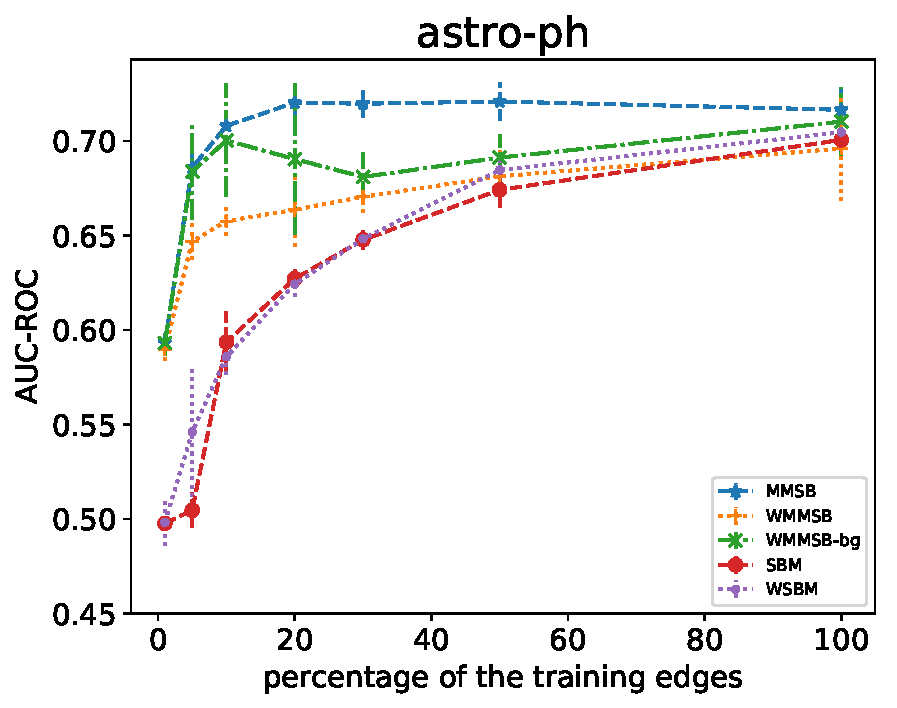
\includegraphics[width=0.32\textwidth]{fig/astro-ph__entropy@_roc_evo}
\end{subfigure}
\begin{subfigure}
         \centering
      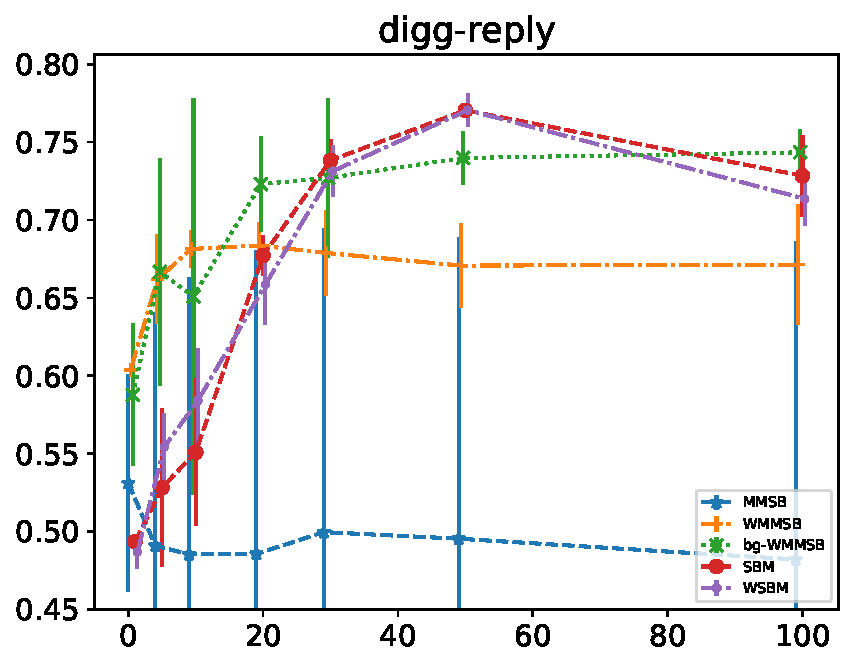
\includegraphics[width=0.32\textwidth]{fig/digg-reply__entropy@_roc_evo}               
\end{subfigure}                                                                          
\begin{subfigure}                                                                        
         \centering                                                                      
      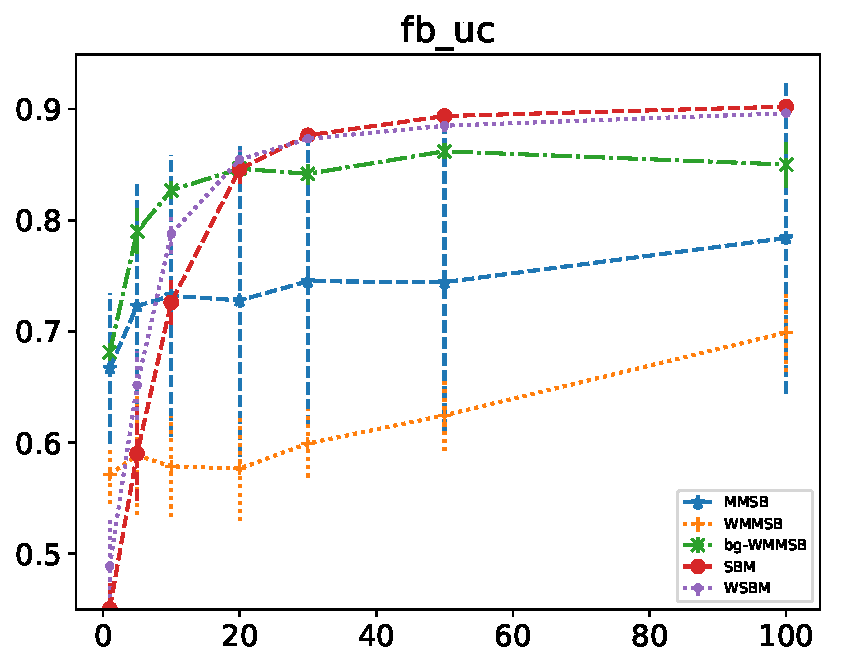
\includegraphics[width=0.32\textwidth]{fig/fb_uc__entropy@_roc_evo}
\end{subfigure}                                                                          
\begin{subfigure}                                                                        
         \centering                                                                      
      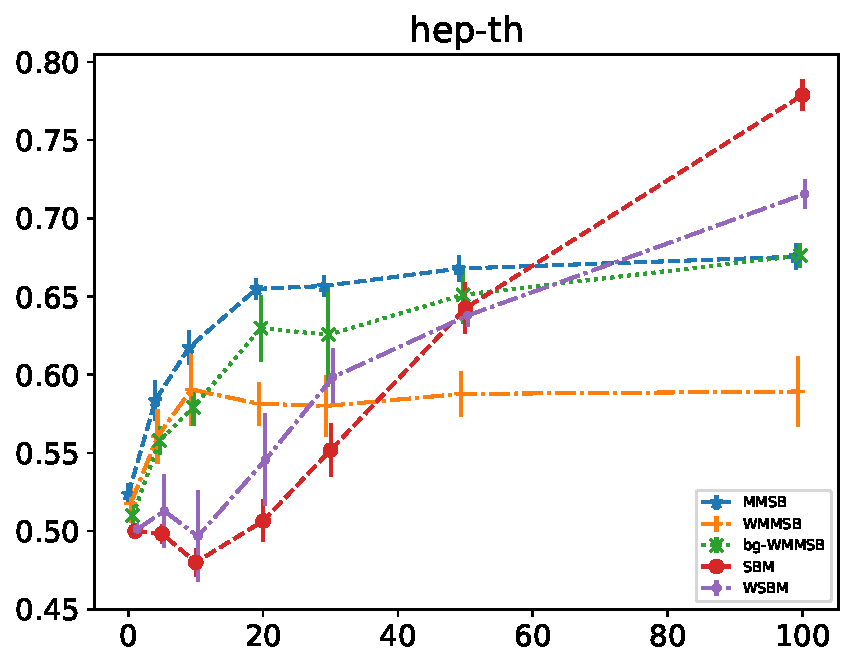
\includegraphics[width=0.32\textwidth]{fig/hep-th__entropy@_roc_evo}
\end{subfigure}                                                                          
\begin{subfigure}                                                                        
     \centering                                                                          
         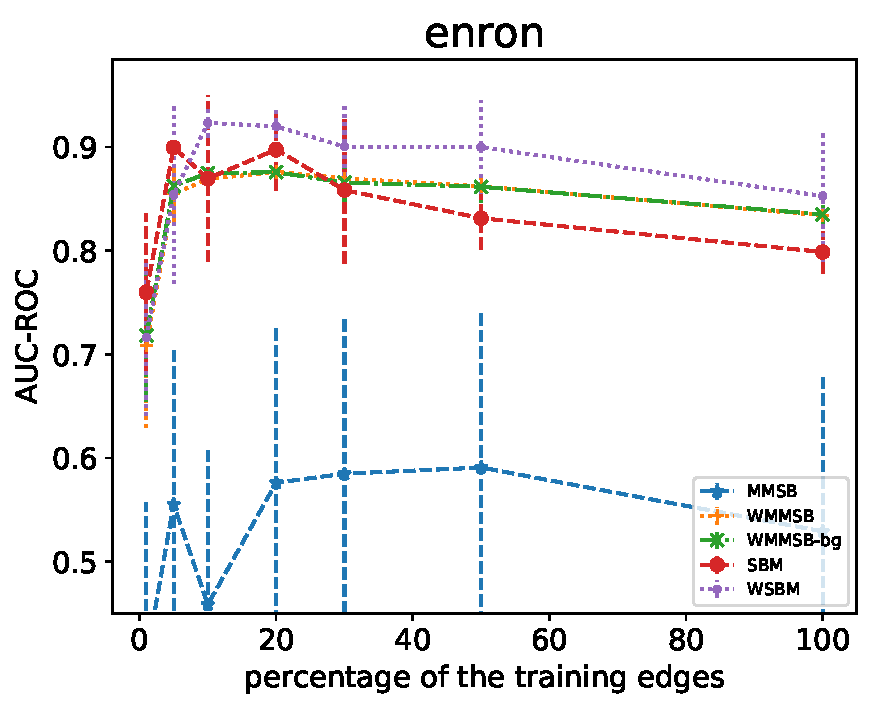
\includegraphics[width=0.32\textwidth]{fig/enron__entropy@_roc_evo}
\end{subfigure}
\begin{subfigure}
         \centering
      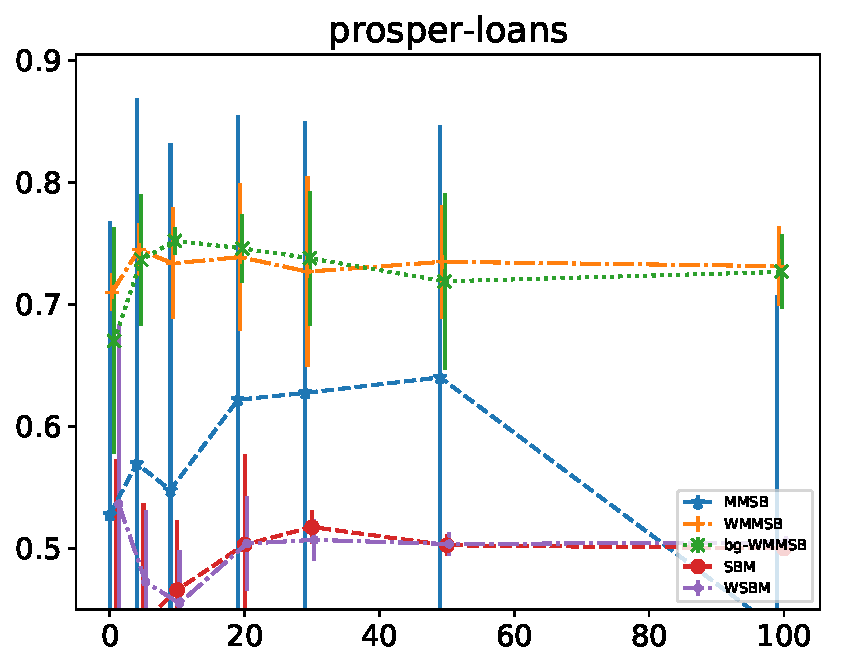
\includegraphics[width=0.32\textwidth]{fig/prosper-loans__entropy@_roc_evo}
\end{subfigure}                                                             
\begin{subfigure}                                                           
         \centering                                                         
      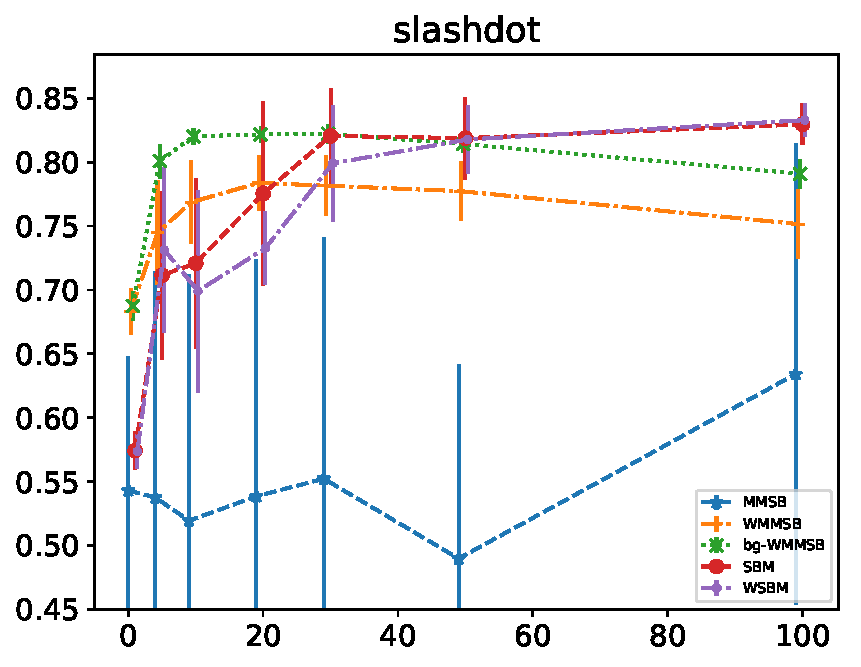
\includegraphics[width=0.32\textwidth]{fig/slashdot__entropy@_roc_evo}
\end{subfigure}                                                             
\begin{subfigure}                                                           
         \centering                                                         
      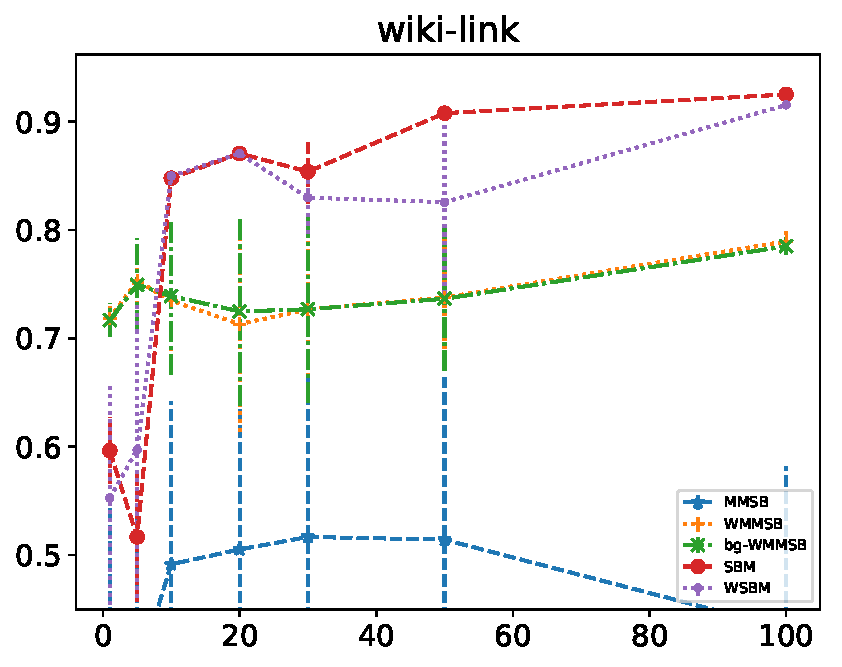
\includegraphics[width=0.32\textwidth]{fig/wiki-link__entropy@_roc_evo}
\end{subfigure}                                                             
\begin{subfigure}                                                           
         \centering                                                         
      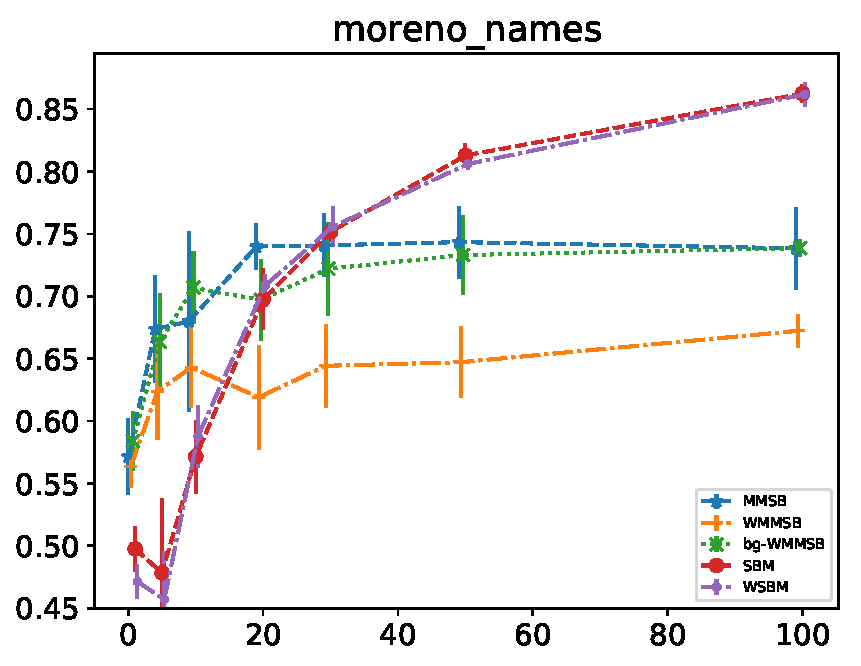
\includegraphics[width=0.32\textwidth]{fig/moreno_names__entropy@_roc_evo}
\end{subfigure}                                                             
\caption{Comparison of models in terms of AUC-ROC scores according to the percentage of edges used to train the models (from 1 to 100\%).}


   \label{fig:roc}
\end{figure}


\begin{figure}[h]
\centering
	
\begin{subfigure}
     \centering
         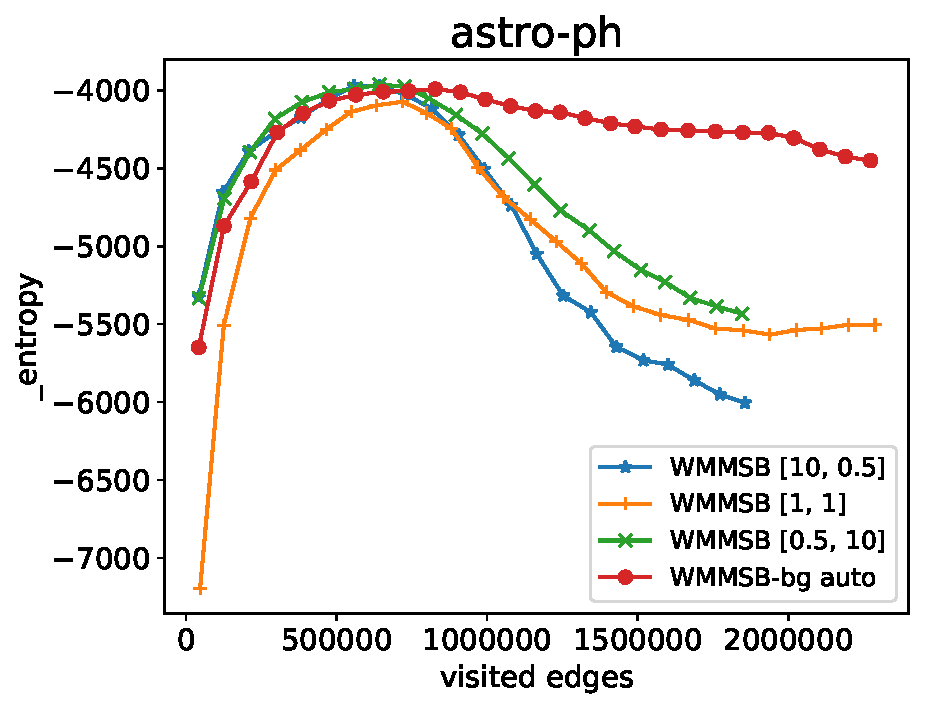
\includegraphics[width=0.32\textwidth]{fig/astro-ph_fig__entropy}
\end{subfigure}
\begin{subfigure}
         \centering
      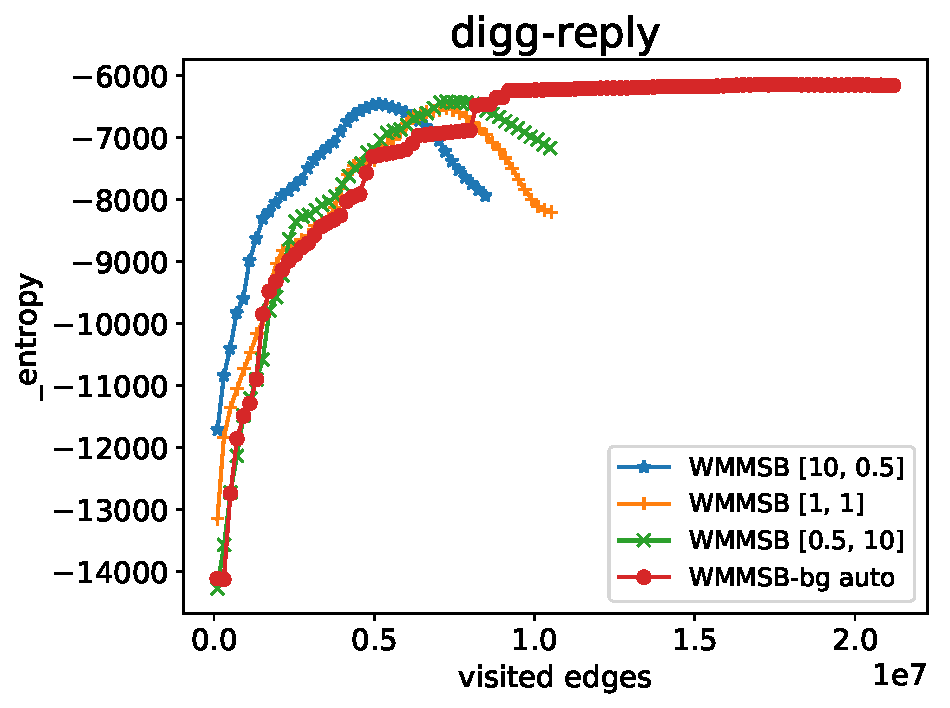
\includegraphics[width=0.32\textwidth]{fig/digg-reply_fig__entropy}               
\end{subfigure}                                                                          
\begin{subfigure}                                                                        
         \centering                                                                      
      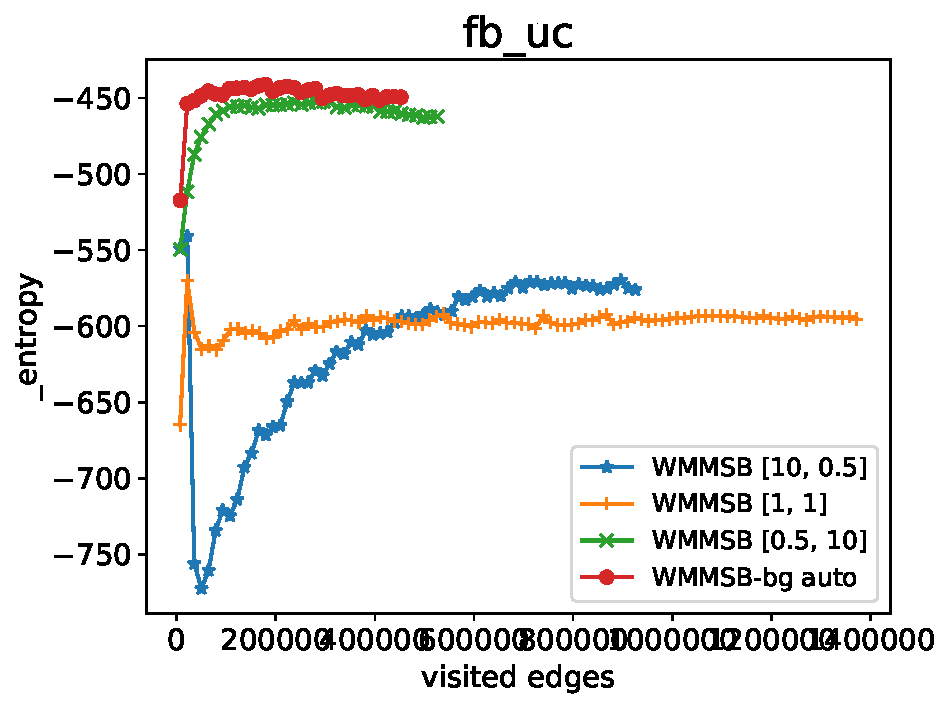
\includegraphics[width=0.32\textwidth]{fig/fb_uc_fig__entropy}
\end{subfigure}                                                                          
\begin{subfigure}                                                                        
         \centering                                                                      
      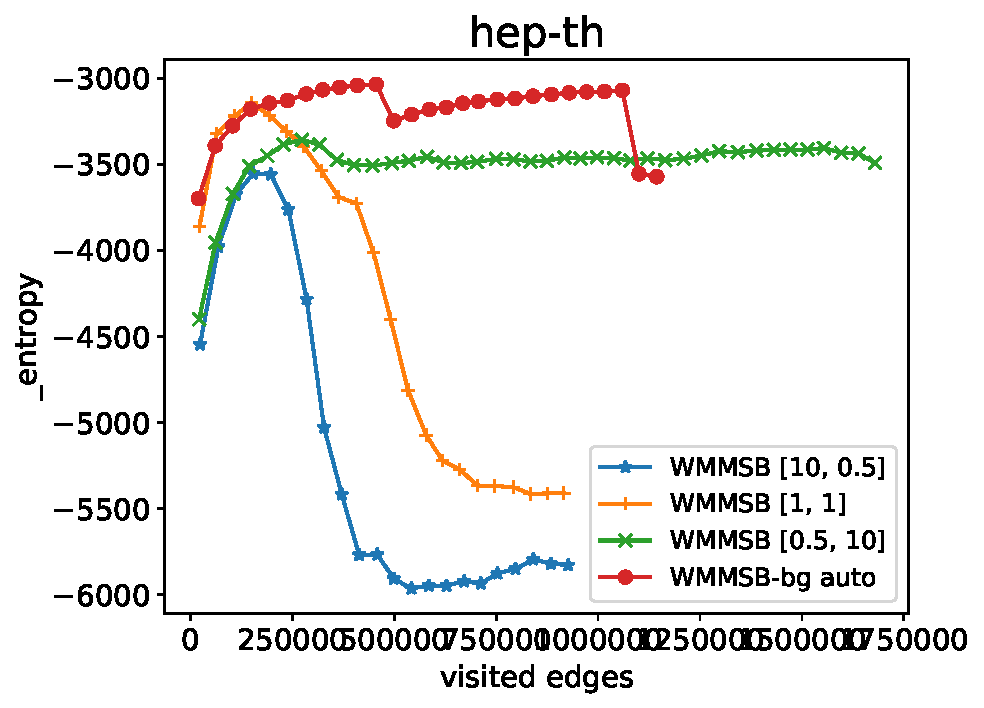
\includegraphics[width=0.32\textwidth]{fig/hep-th_fig__entropy}
\end{subfigure}                                                                          
\begin{subfigure}                                                                        
     \centering                                                                          
         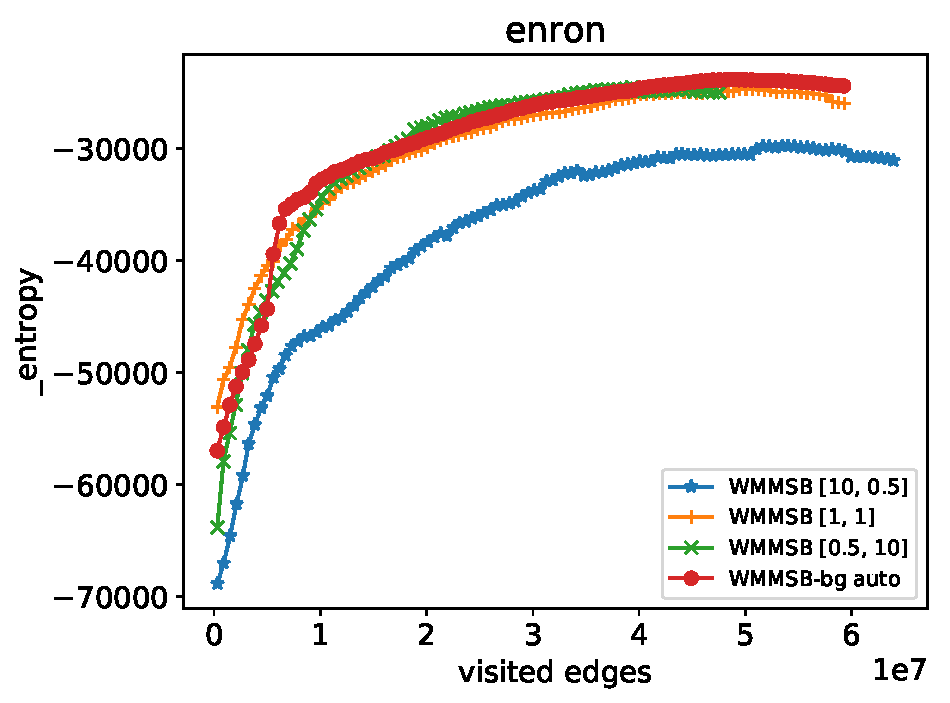
\includegraphics[width=0.32\textwidth]{fig/enron_fig__entropy}
\end{subfigure}
\begin{subfigure}
         \centering
      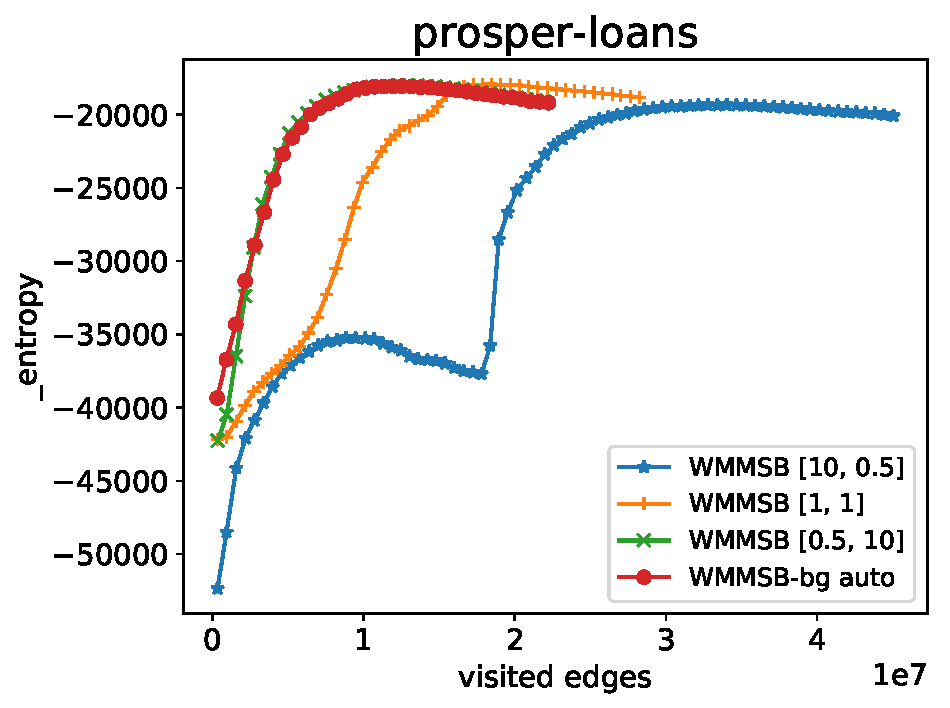
\includegraphics[width=0.32\textwidth]{fig/prosper-loans_fig__entropy}
\end{subfigure}                                                             
\begin{subfigure}                                                           
         \centering                                                         
      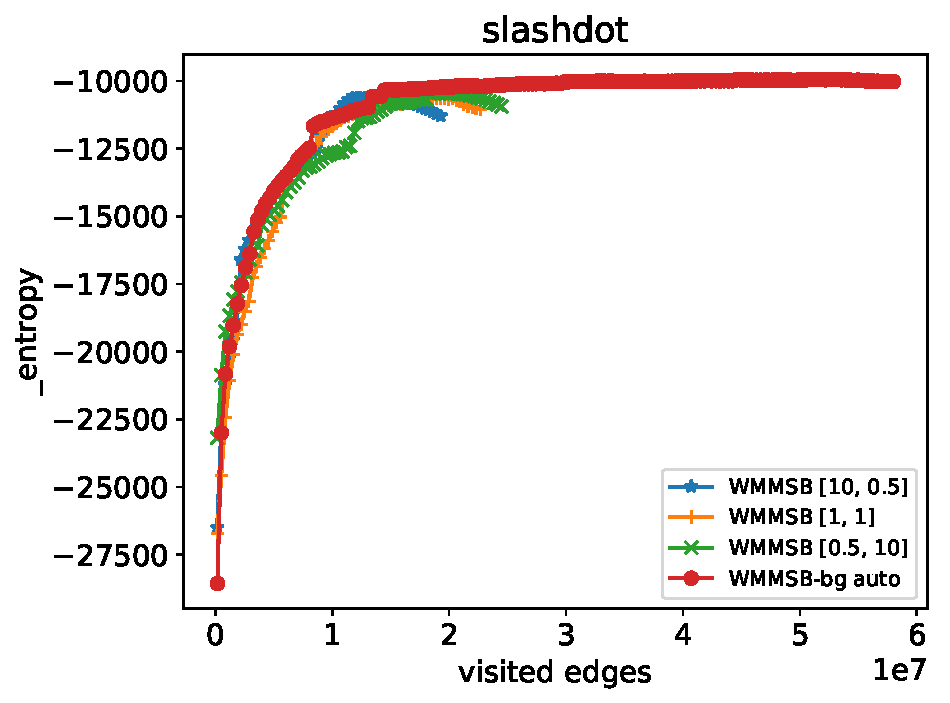
\includegraphics[width=0.32\textwidth]{fig/slashdot_fig__entropy}
\end{subfigure}                                                             
\begin{subfigure}                                                           
         \centering                                                         
      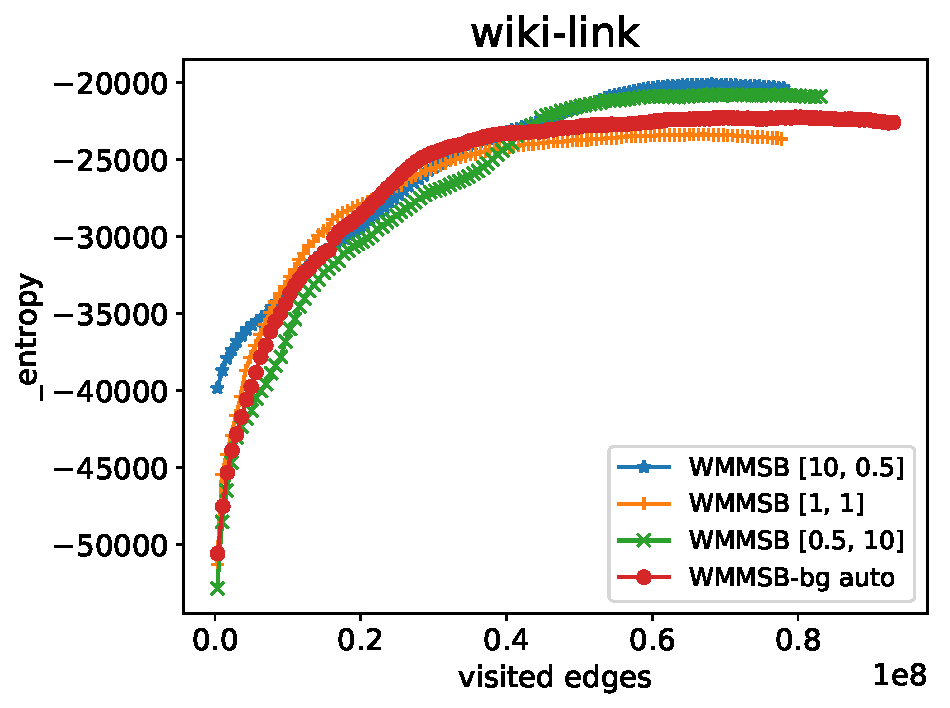
\includegraphics[width=0.32\textwidth]{fig/wiki-link_fig__entropy}
\end{subfigure}                                                             
\begin{subfigure}                                                           
         \centering                                                         
      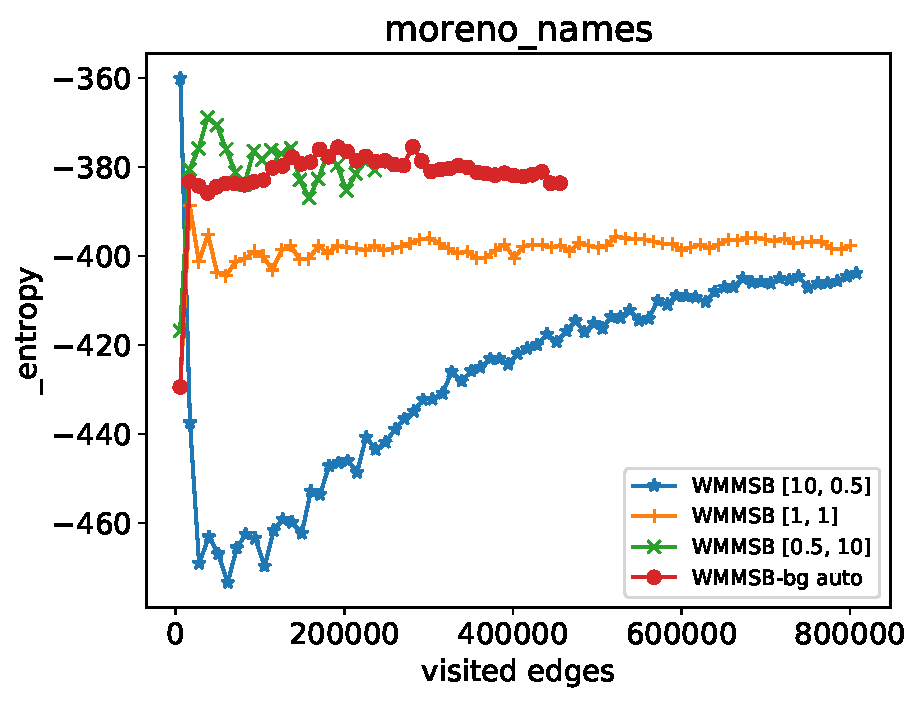
\includegraphics[width=0.32\textwidth]{fig/moreno_names_fig__entropy}
\end{subfigure}                                                             
\caption{Log-likehood convergence for WMMSB and WMMSB-bg models. Three different sets of hyper-parmeter are used for WMMSB.}


    \label{fig:conv_entropy}
\end{figure}

\section{Reproducible Research}

We published our implementation within a platform that aims to ease the development of reproducible complex experiments. We are maintaining this platform that we released under open-source license.\footnote{The name of the project is anonymized.}

To reproduce our results, one can proceed as follows:
\begin{itemize}
\item Install the XXX project:   %\lstinline|git clone https://github.com/*/XXX|  
    \begin{lstlisting}[language=bash]
          $ git clone https://github.com/*/*
          $ cd XXX and make install
    \end{lstlisting}
\item Fit all the models on all the corpus, and save the results:
\begin{lstlisting}[language=bash]
        $ XXX online_roc -x fit -w --repeat 0 1 2 3 4 5 6 7 8 9 
\end{lstlisting}
\item Parallelization can be obtained by adding the options \lstinline|--cores NUMBER_OF_CORES|,
\item Figures can be plotted with the command:  
\begin{lstlisting}[language=bash]
        $ XXX online_roc -x roc_evolution2 --repeat 0 1 2 3 4 5 6 7 8 9
\end{lstlisting}
\end{itemize}



\clearpage
\bibliographystyle{unsrt}
%\bibliographystyle{splncs04}

\bibliography{./a}

%\clearpage
%\appendix
%\section{Derivation of the collapsed variational updates}

The derivation of the collapsed variational updates is first obtained by maximizing the ELBO w.r.t $\gamma_{ijkk'}$ with:
%
\begin{align*}
\frac{\partial \L_Z}{\partial \gamma_{ijkk'}} &= \frac{\partial }{\partial \gamma_{ijkk'}}  \sum_{Z^{-ij}}\sum_{k_1=1}^K\sum_{k_2=1}^K  q(Z^{-ij}) \gamma_{ijk_1 k_2} (\log p(Y, Z^{-ij}, z_{i\rightarrow j}=k_1, z_{i\leftarrow j}=k_2|\Omega)+ \\
& \qquad \log q(Z^{-ij}, z_{i\rightarrow j}=k_1, z_{i\leftarrow j}=k_2) )   \\
&= E_{q(Z^{-ij})}[ p(Y, Z^{-ij}, z_{i\rightarrow j}=k, z_{i\leftarrow j}=k'|\Omega))] + H[Z^{-ij}] -\log(\gamma_{ijkk'}) +1
\end{align*}
%
By equating this derivative to zero, one obtains the following update:
\begin{equation} \label{eq1}
\gamma_{ijkk'} \propto \exp E_{q(Z^{-ij})} [\log P(z_{i\rightarrow j}=k, z_{i\leftarrow j}=k' | Y^{-ij}, Z^{-ij}, \Omega) ]
\end{equation}
%
with  $P(z_{i\rightarrow j}=k, z_{i\leftarrow j}=k' | Y^{-ij}, Z^{-ij}, \Omega)$ being the collapsed Gibbs update of WMMSB, of the form:
%
\begin{align*}
P(z_{i\rightarrow j}=k, z_{i\leftarrow j}=k' |Y^{-ij}, Z^{-ij}, \Omega) \propto (n_{\rightarrow ik}^{\Theta^{-j}} + \alpha_k) (n_{\leftarrow jk}^{\Theta^{-i}} + \alpha_{k'}) \mathrm{NB}\left(y_{ij}; n^{Y^{-ij}}_{kk'} + r, \frac{p}{p\,n^{\Phi^{-ij}}_{\bm{.}kk'} + 1} \right)
\end{align*}
%
with count statistics given by the following equations:

%\begin{align} \label{eq:sss}
%    n^{\Theta}_{\rightarrow ik} &= \sum_{j, k'} \gamma_{ijkk'}        & n^{\Theta}_{\leftarrow jk'} &= \sum_{i, k} \gamma_{ijkk'}  \nonumber \\
%    n^{\Phi}_{xkk'} &= \sum_{ij:y_{ij}=x} \gamma_{ijkk'}  & n^{Y}_{kk'} &= \sum_{ij} y_{ij}\gamma_{ijkk'}
%\end{align}

\begin{align*}                                                                                                                                        
&n^{\Theta}_{\rightarrow ik} = \sum_j \delta(\zij=k)\\
&n^{Y}_{kk'} = \sum_{ij} y_{ij}\delta(\zij=k, \zji=k') \\
&n^{\Phi}_{\bm{.}kk'} = \sum_{ij} \delta( \zij=k, \zji=k') 
\end{align*}   

By applying a first order Taylor expansion on Eq.~\eqref{eq1}, following \cite{teh2007collapsed}, one obtains:

\begin{equation}
\gamma_{ijkk'} \propto (E_{q(Z^{-ij})}[n_{\rightarrow ik}^{\Theta^{-j}}] + \alpha_k) (E_{q(Z^{-ij})}[n_{\leftarrow jk}^{\Theta^{-i}}] + \alpha_{k'}) \mathrm{NB}\left(y_{ij}; E_{q(Z^{-ij})}[n^{Y^{-ij}}_{kk'}] + r, \frac{p}{p\,E_{q(Z^{-ij})}[n^{\Phi^{-ij}}_{\bm{.}kk'}] + 1} \right) \nonumber
\end{equation}

Finally, using a Gaussian approximation (as in \textit{e.g.} \cite{asuncion2009smoothing}), one can estimate the expectations $E_{q(Z^{-ij})}[n_{\rightarrow ik}^{\Theta^{-j}}], E_{q(Z^{-ij})}[n_{\leftarrow jk}^{\Theta^{-i}}]$ and  $E_{q(Z^{-ij})}[n^{\Phi^{-ij}}_{\bm{.}kk'}]$ with the counts defined in Eq. 2 of Section 3.1.

\section{Beta-Gamma updates}

In the WMMSB-bg model, the collapsed variational distribution takes the form:

\begin{equation*}
q(\Pi) = q(\Theta, \Phi|Z, R, P) q(Z)q(R)q(P)
\end{equation*}

The variational distribution for $r_{kk'}$ is taken in the Gamma family:  $q(r_{kk'}) = \textrm{Gamma}(a_{kk'},b_{kk'})$ for $1\leq k,k' \leq K$. The collapsed ELBO can thus be rewritten as:

\begin{align*}
\log p(Y) \geq \L_{Z,R,P} &= \E_{q}[\log p(Y, Z, R, P|\Omega)] + \textrm{H}[q(Z)] + \textrm{H}[q(R)] + \textrm{H}[q(P)] \\
                        &= \E_{q}[\log p(Y, Z)] + \textrm{H}[q(Z)] \\
                        &\qquad + \E_{q}[\log p(R|Y,Z,P)] + \textrm{H}[q(R)] \\
                        &\qquad +\E_{q}[\log p(P|Y,Z)] + \textrm{H}[q(P)] 
\end{align*}

\paragraph{Optimizing $\gamma_{ijkk'}$}

In the Beta-Gamma augmentation, the parameters $p$ and $r$ are marginalized in the update given by Eq.~\eqref{eq1}:
\begin{equation}
\gamma_{ijkk'} \propto \exp E_{q(Z^{-ij})} [\log E_{q(r_{kk'})}[E_{q(p_{kk'})}[ P(z_{i\rightarrow j}=k, z_{i\leftarrow j}=k' | Y^{-ij}, Z^{-ij}, \Omega) ] ] ] \nonumber
\end{equation}

By using a first order Taylor expansion, one obtains:

\begin{equation}
\gamma_{ijkk'} \propto (N_{\rightarrow ik}^{\Theta^{-j}} + \alpha_k) (N_{\leftarrow jk}^{\Theta^{-i}} + \alpha_{k'}) \mathrm{NB}\left(y_{ij}; N^{Y^{-ij}}_{kk'} + \E_{q}[r_{kk'}], \frac{\E_{q}[p_{kk'}]}{\E_{q}[p_{kk'}]\,N^{\Phi^{-ij}}_{\bm{.}kk'} + 1} \right) \nonumber
\end{equation}

\paragraph{Optimizing $r_{kk'}$}

We isolate the part of the ELBO than depends only on $r_{kk'}$ parameters ($a_{kk'}$ and $b_{kk'}$). Thus, we consider only the links that have been generated within the classes $k,k'$, denoted by $Y^{(kk')}$. Furthermore, as $y_{ij} \sim NB(r_{kk'}, p_{kk'})$ if $i$ is in class $k$ and $j$ in class $k'$, one has:

\begin{align*}
\L_{[r_{kk'}]} = \E_{q(r_{kk'})}[\log p(r_{kk'}|Y^{(kk')},Z^{(kk')},p_{kk'})] + \textrm{H}[q(r_{kk'})] \\
\end{align*}

By applying Bayes rules and dropping the normalizing term that does not depend on $r_{kk'}$, one gets:

\begin{align*}
\L_{[r_{kk'}]} &= \E_{q(r_{kk'})}[\log \left( p(Y^{(kk')}|Z^{(kk')}, r_{kk'}, p_{kk'}) p(r_{kk'}]) \right)] + \textrm{H}[q(r_{kk'})] \\
    &= \E_{q(r_{kk'})}[\log \left( \prod_{ij\in Y^{(kk')}} \dbinom{r_{kk'} + y_{ij}-1}{y_{ij}} (1-p_{kk'})^{r_{kk'}} p_k^{y_{ij}} p(r_{kk'}) \right) ] + \textrm{H}[q(r_{kk'})] \\
    &= \E_{q(r_{kk'})}[\log \left( (1-p_{kk'})^{r_{kk'} N^{\Phi}_{kk'}} p_{kk'}^{N^{Y}_{kk'}} p(r_{kk'}) \prod_{ij\in Y^{(kk')}} \frac{\Gamma(r_{kk'}+y_{ij})}{\Gamma(r_{kk'}) \Gamma(y_{ij}+1) }  \right) ] + \textrm{H}[q(r_{kk'})]
\end{align*}

If $y_{ij} = 0$, then $\frac{\Gamma(r_{kk'}+y_{ij})}{\Gamma(r_{kk'}) \Gamma(y_{ij}+1)} = 1$, whereas if $y_{ij} \ne 0$, then $\frac{\Gamma(r_{kk'}+y_{ij})}{\Gamma(r_{kk'}) \Gamma(y_{ij}+1)} = \frac{1}{B(r_{kk'}, y_{ij})y_{ij}}$. Furthermore, in this latter case:
%
\begin{align*}
B(r_{kk'}, y_{ij}) = \int_0^1 t^{r_{kk'}-1} (1-t)^{y_{ij}-1} dt  \leq \int_0^1 t^{r_{kk'}-1} dt = \frac{1}{r_k}
\end{align*}
%
so that:
%
\begin{equation*}
\log \prod_{ij\in Y^{(kk')}} \frac{\Gamma(r_{kk'}+y_{ij})}{\Gamma(r_{kk'}) \Gamma(y_{ij}+1) } \geq N^Y_{kk'} \log(r_{kk'}) + \mathrm{cst}
\end{equation*}
%
with $N^Y_{kk'} = \sum_{ij\in Y^{(kk')}} y_{ij}$.

Furthermore, from the model definitions, one has: $\log p(r_{kk'}) = (r_0 c_0-1)\log(r_{kk'}) - r_{kk'} c_0 + \mathrm{cst}$  and $\textrm{H}[q(r_{kk'})] = a_{kk'} + \log(b_{kk'}) +\log \Gamma(a_{kk'}) + (1-a_{kk'})\Psi(a_{kk'})$.

Hence:
%
\begin{align*}
\L_{[r_{kk'}]} &\geq N^\Phi_{kk'} a_{kk'} b_{kk'} \log(1-p_{kk'}) + (r_0 c_0-1 )(\Psi(a_{kk'}) + \log(b_{kk'})) -c_0 a_{kk'} b_{kk'} +N^Y_{kk'} (\Psi(a_{kk'}) + \log(b_{kk'}))  \\
&\qquad a_{kk'} + \log(b_{kk'}) +\log \Gamma(a_{kk'}) + (1-a_{kk'})\Psi(a_{kk'})
\end{align*}

Maximizing the right-hand term of the above inequality with respect to $b_{kk'}$ yields:

\begin{equation} \label{eq:update2}
b_{kk'} = \frac{r_0 c_0 + N^Y_{kk'}}{a_{kk'} (c_0 - N^\Phi_{kk'} \log(1-p_{kk'}))} \nonumber
\end{equation}

As $r_{kk'} \sim \textrm{Gamma}(a_{kk'},b_{kk'})$, one finally obtains:

\begin{equation}
\E_q[r_{kk'}] = a_{kk'} b_{kk'} = \frac{r_0 c_0 + N^Y_{kk'}}{c_0 - N^\Phi_{kk'} \log(1-p_{kk'})} \nonumber
\end{equation}

\paragraph{Optimizing $p_{kk'}$}

In oder to maximize the ELBO w.r.t $p_{kk}'$, one can let $q(p_{kk'}) = p(p_{kk'} | Y,Z) = E_q(r_{kk'}) [ p(p_{kk'} | Y^{(kk')},Z^{(kk')} ,r_{kk'})]$. As the negative binomial and Beta distributions are conjugate, a closed-form expression can be obtained:

\begin{align*}
p(p_{kk'} | Y^{(kk')}, Z^{(kk')}, r_{kk'}) &\propto p(Y^{(kk')| Z^{(kk')}, r_{kk'}} p(r_{kk'}) \\
                               &\propto (1-p_{kk'})^{r_{kk'} N^\Phi_{kk'}}p_{kk'}^{N^Y_{kk'}} p_{kk'}^{c\epsilon -1} (1-p_{kk'})^{c(1-\epsilon) -1}\\
                               &\propto p_{kk'}^{c\epsilon + N^Y_{kk'} -1} (1-p_{kk'})^{c(1-\epsilon) + N^\Phi_{kk'}r_{kk'}-1}\\
                               &= \mathrm{Beta}(c\epsilon + N^Y_{kk'}, c(1-\epsilon) + N^\Phi_{kk'}r_{kk'})
\end{align*}

Finally, by resorting again to a first order Taylor expansion, one obtains:

\begin{equation*}
p_{kk'} \sim \mathrm{Beta}(c\epsilon + N^Y_{kk'}, c(1-\epsilon) + N^\Phi_{kk'} E_q[r_{kk'}]) \nonumber
\end{equation*}


%\section{Stratified Sampling}
%
%Sampling from minibatches in SVI, for MMSB model, was initially proposed in [6] and [7]. The adaptation of the sampling scheme for SCVI is based on the reformulation of the "sufficient statistics" $N^\Theta, N^\Phi$ and $N^Y$  by bringing up a minibatch distribution $h(S)$. The idea of the stratified sampling is to divide the edges into subset that share some statistical strength.
%For each node $n$ with divide it's neighbors pairs into a set $S_1$ containing all its links (edges) and a subset $S_0$ dividing into  $m$ set containing its non-links. Then sampling consists of drawing one of its its set $S_0$ or $S_0$ with probability.
%
%\begin{align*}
%h(S)=\begin{cases}
%    \frac{1}{2 N}  & \textrm{ if } S = S_1 \\
%    \frac{1}{2 N m}  & \textrm{ if } S \in S_0 
%    \end{cases}
%\end{align*}
%
%
%By referencing any of the global "sufficient statistics" of the models with the term $N^*$ such that $N^* \in \{N^Y, N^\Theta, N^\Phi\}$. Assuming that every pair (i, j) occurs in some constant number of sets c, $N^*$ can be reformulated as follows 
%
%\begin{align*}
%N^* = \sum_{ij, *} \gamma_{ij} = \E_h[ \frac{1}{c}\frac{1}{h(S)} \sum_{ij \in S, *} \gamma_{ij}  ]
%\end{align*}
%
%Where $N^*$ and $\gamma_{ij}$ are matricies of size $K\times K$.
%The exact summing formulation of $N^*=\sum_{ij,*}$ is given in section 3.1. For undirected network, $c$ is equal to 2 because each pair occurs in two set, and $c$ is 1 for directed network.


\section{Experimentation}

We provide here the complete set of results for the AUC-ROC scores evaluations for the full range of training sets proportions (1\%, 5\%, 10\%, 20\%, 30\%, 50\% and 100\%) in Figure \ref{fig:roc} for all the datasets. The log-likelihood convergence of the inference for all the datasets are given in Figure \ref{fig:conv_entropy},

\begin{figure}[h]
\centering
	

\begin{subfigure}
     \centering
         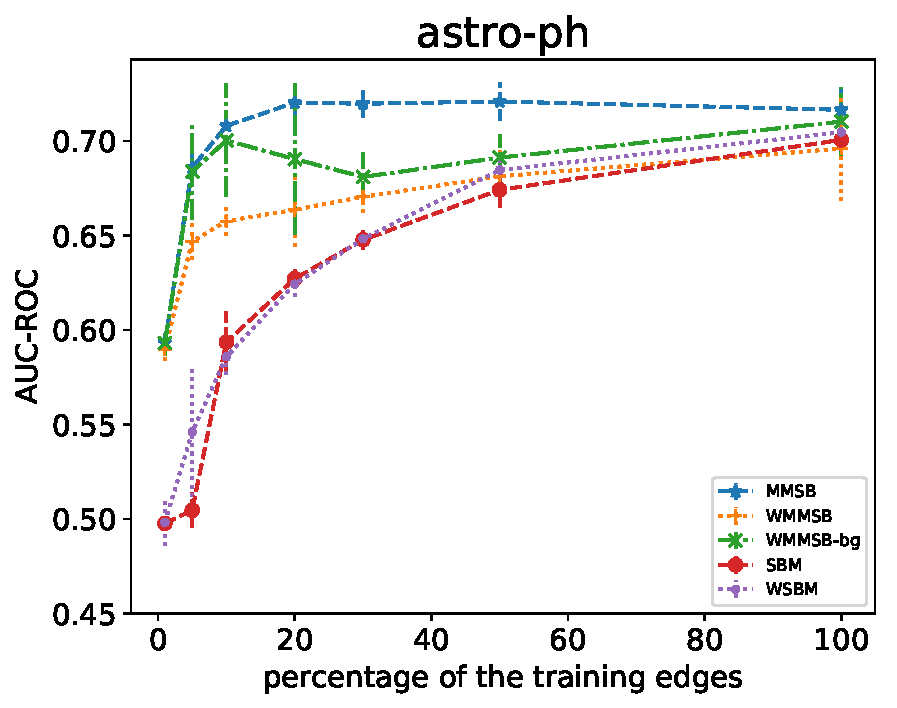
\includegraphics[width=0.32\textwidth]{fig/astro-ph__entropy@_roc_evo}
\end{subfigure}
\begin{subfigure}
         \centering
      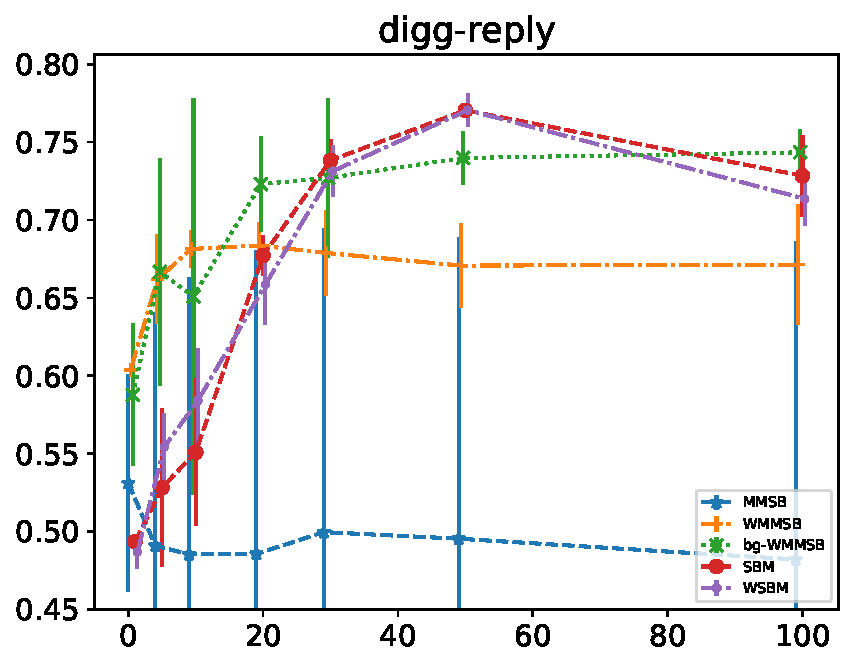
\includegraphics[width=0.32\textwidth]{fig/digg-reply__entropy@_roc_evo}               
\end{subfigure}                                                                          
\begin{subfigure}                                                                        
         \centering                                                                      
      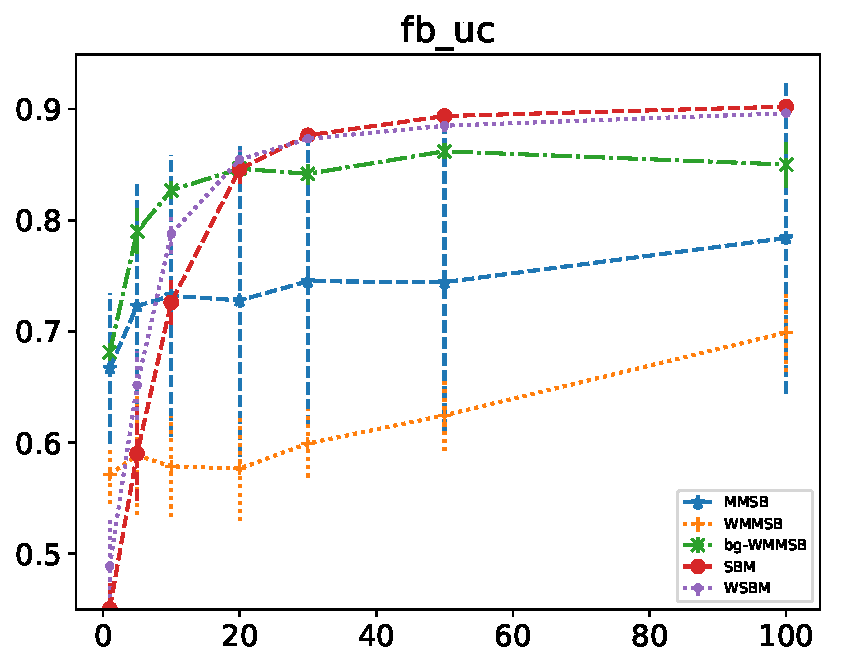
\includegraphics[width=0.32\textwidth]{fig/fb_uc__entropy@_roc_evo}
\end{subfigure}                                                                          
\begin{subfigure}                                                                        
         \centering                                                                      
      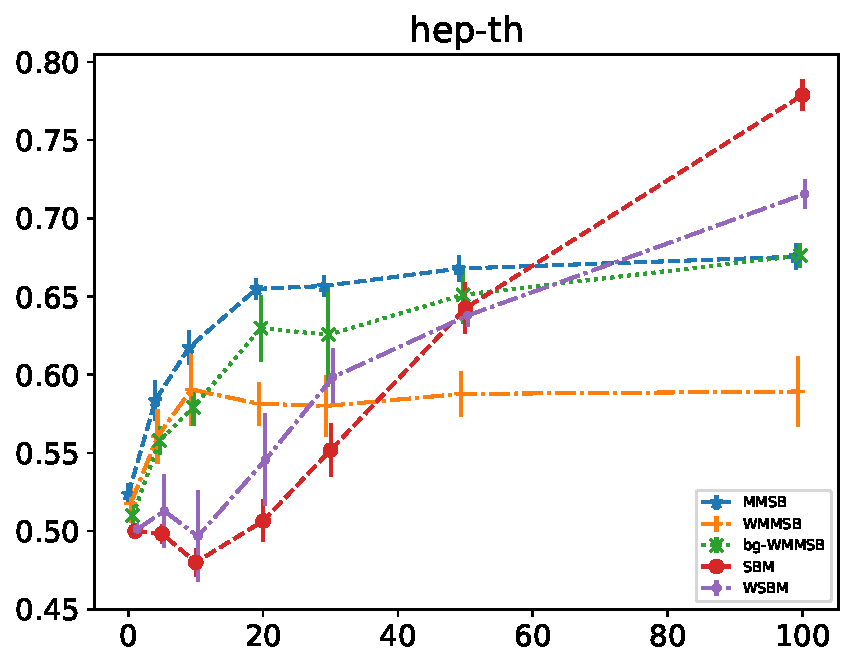
\includegraphics[width=0.32\textwidth]{fig/hep-th__entropy@_roc_evo}
\end{subfigure}                                                                          
\begin{subfigure}                                                                        
     \centering                                                                          
         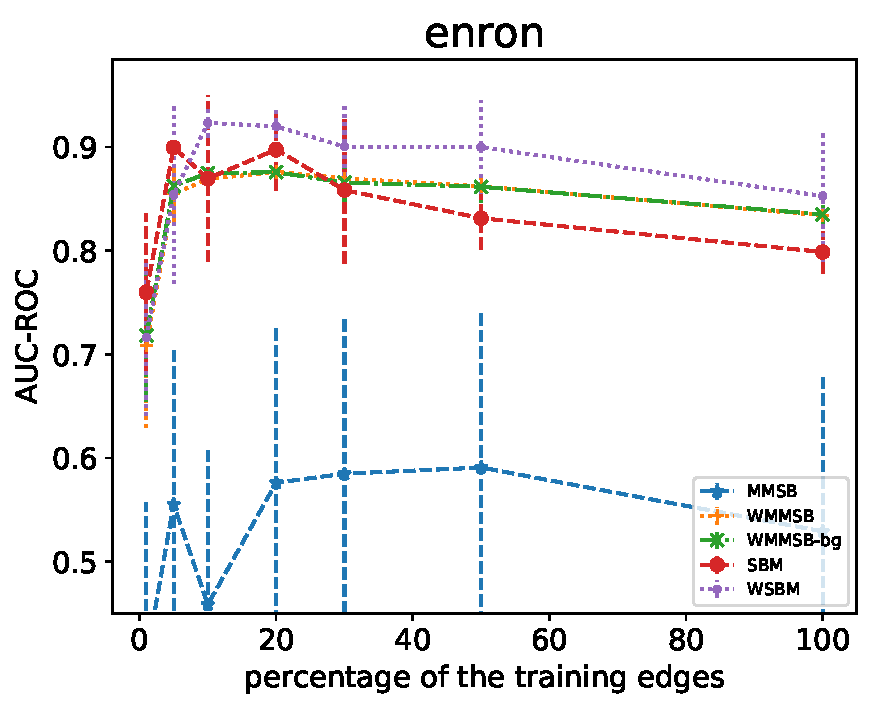
\includegraphics[width=0.32\textwidth]{fig/enron__entropy@_roc_evo}
\end{subfigure}
\begin{subfigure}
         \centering
      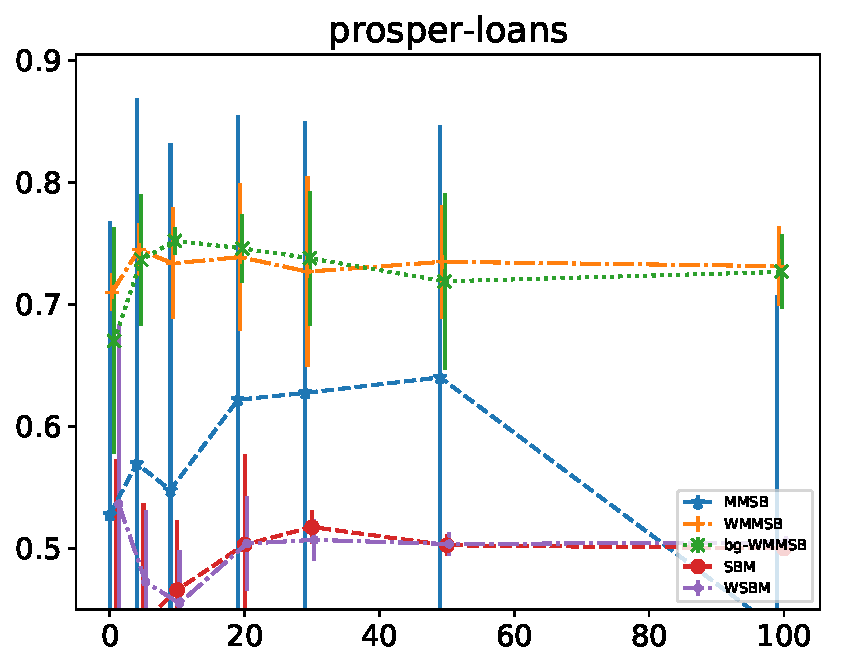
\includegraphics[width=0.32\textwidth]{fig/prosper-loans__entropy@_roc_evo}
\end{subfigure}                                                             
\begin{subfigure}                                                           
         \centering                                                         
      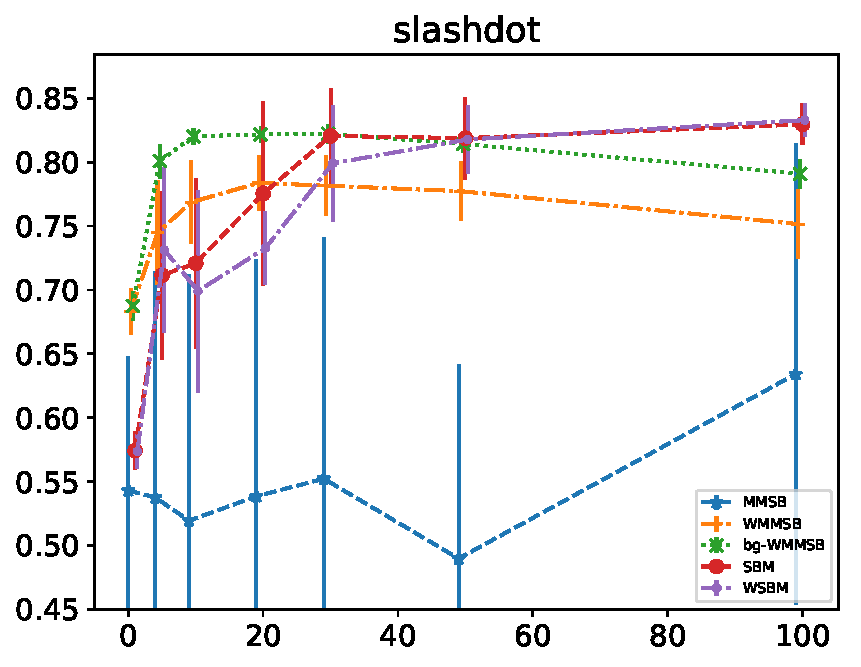
\includegraphics[width=0.32\textwidth]{fig/slashdot__entropy@_roc_evo}
\end{subfigure}                                                             
\begin{subfigure}                                                           
         \centering                                                         
      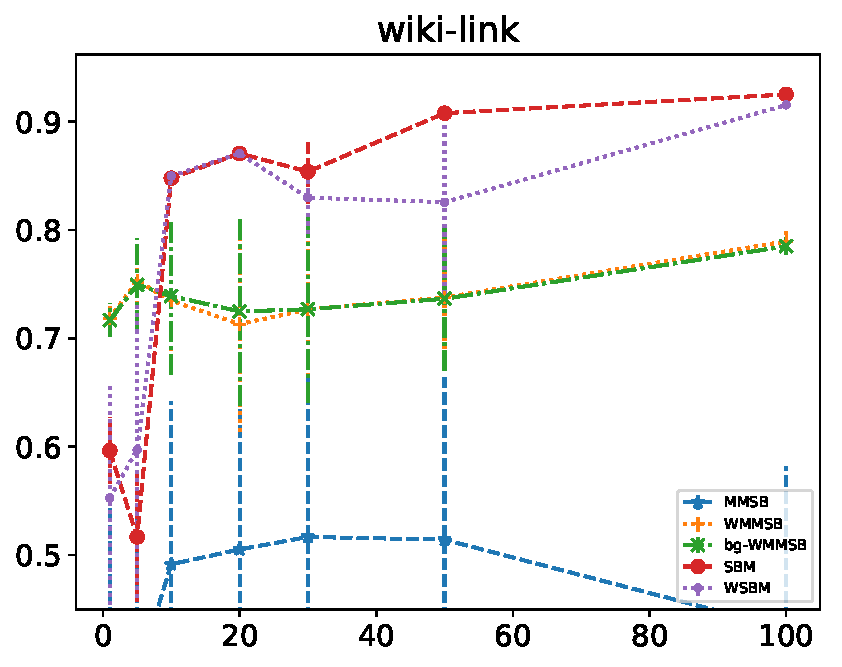
\includegraphics[width=0.32\textwidth]{fig/wiki-link__entropy@_roc_evo}
\end{subfigure}                                                             
\begin{subfigure}                                                           
         \centering                                                         
      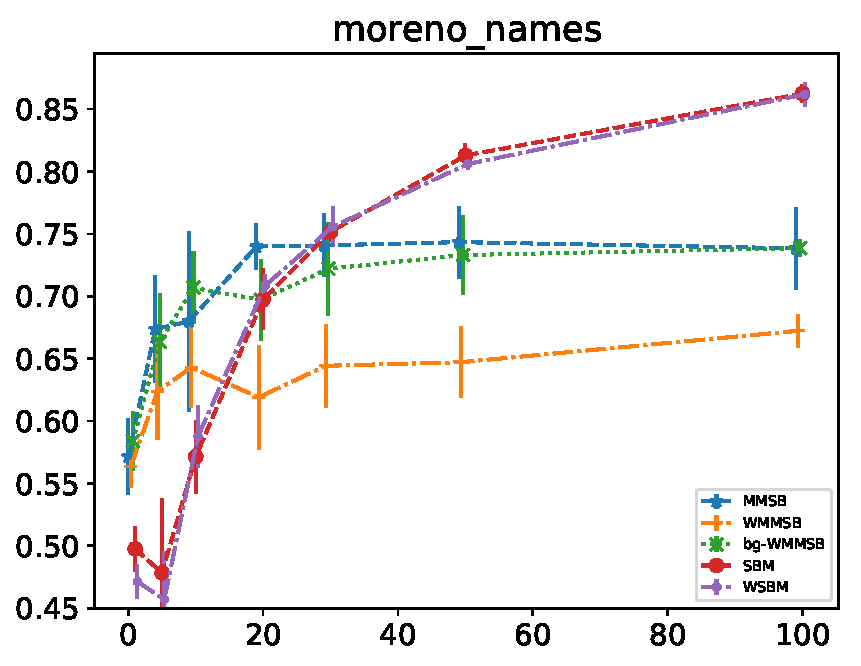
\includegraphics[width=0.32\textwidth]{fig/moreno_names__entropy@_roc_evo}
\end{subfigure}                                                             
\caption{Comparison of models in terms of AUC-ROC scores according to the percentage of edges used to train the models (from 1 to 100\%).}


   \label{fig:roc}
\end{figure}


\begin{figure}[h]
\centering
	
\begin{subfigure}
     \centering
         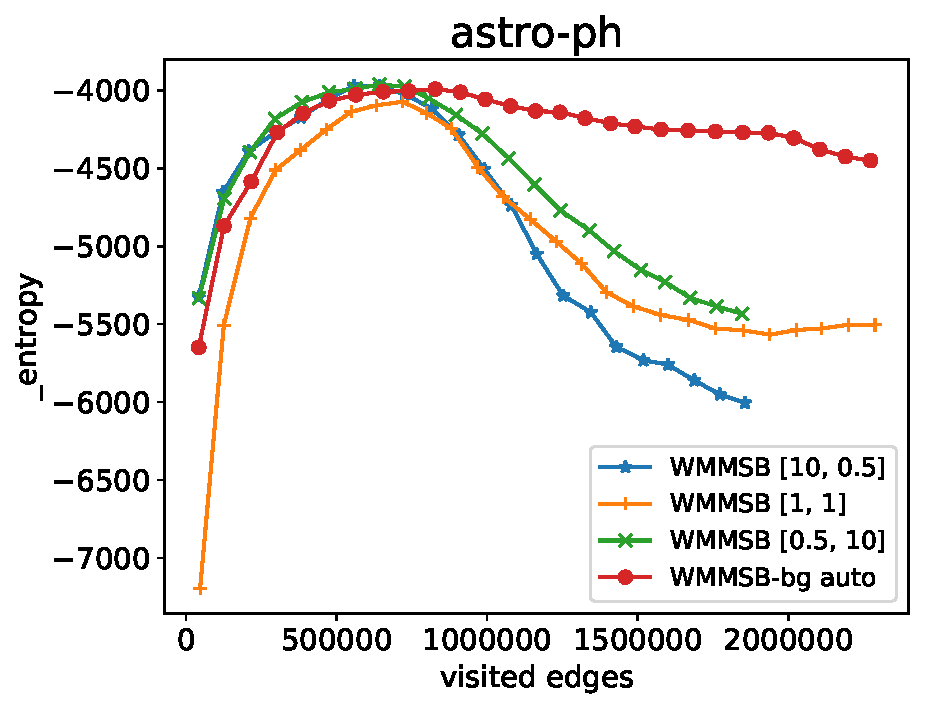
\includegraphics[width=0.32\textwidth]{fig/astro-ph_fig__entropy}
\end{subfigure}
\begin{subfigure}
         \centering
      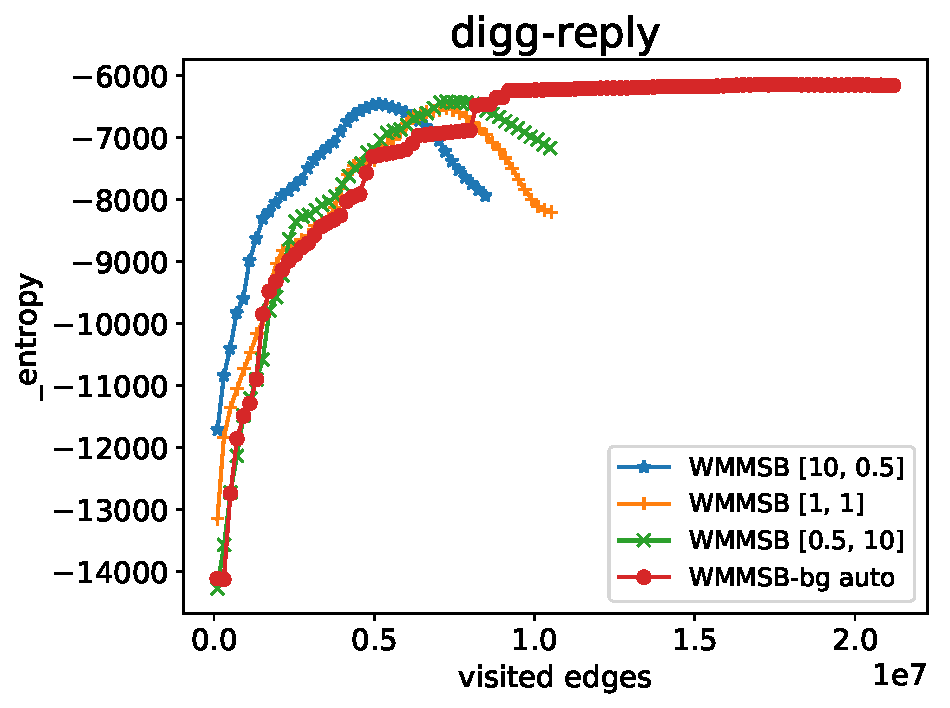
\includegraphics[width=0.32\textwidth]{fig/digg-reply_fig__entropy}               
\end{subfigure}                                                                          
\begin{subfigure}                                                                        
         \centering                                                                      
      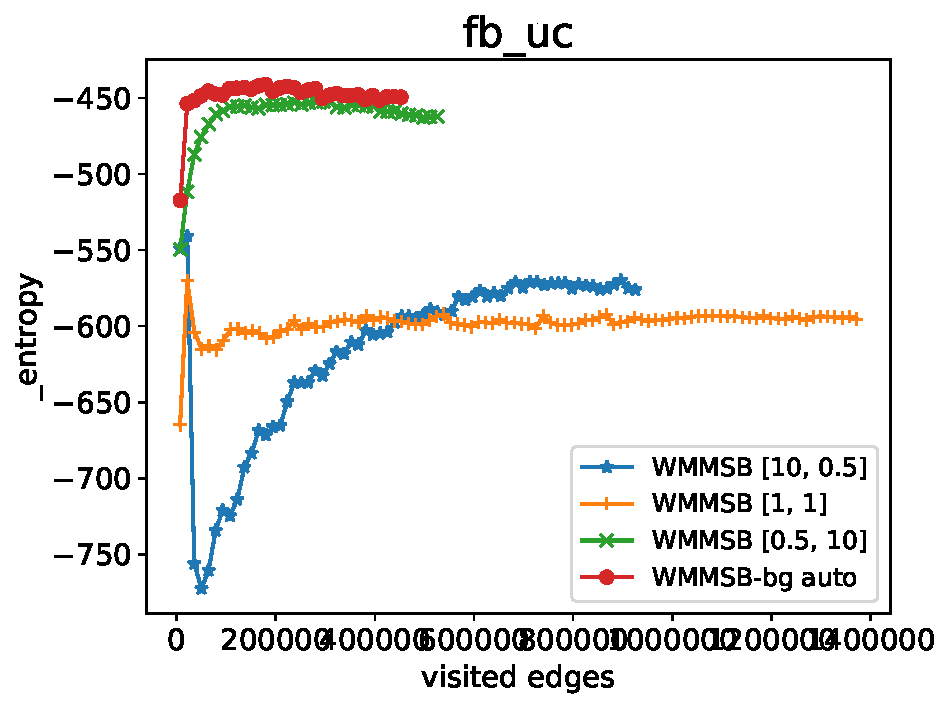
\includegraphics[width=0.32\textwidth]{fig/fb_uc_fig__entropy}
\end{subfigure}                                                                          
\begin{subfigure}                                                                        
         \centering                                                                      
      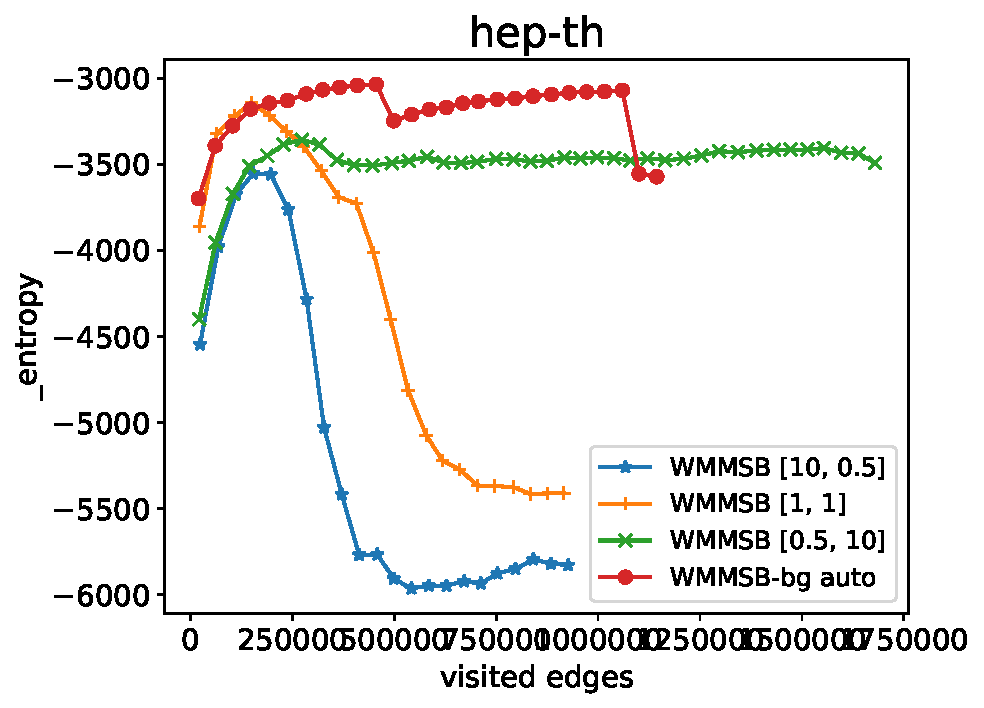
\includegraphics[width=0.32\textwidth]{fig/hep-th_fig__entropy}
\end{subfigure}                                                                          
\begin{subfigure}                                                                        
     \centering                                                                          
         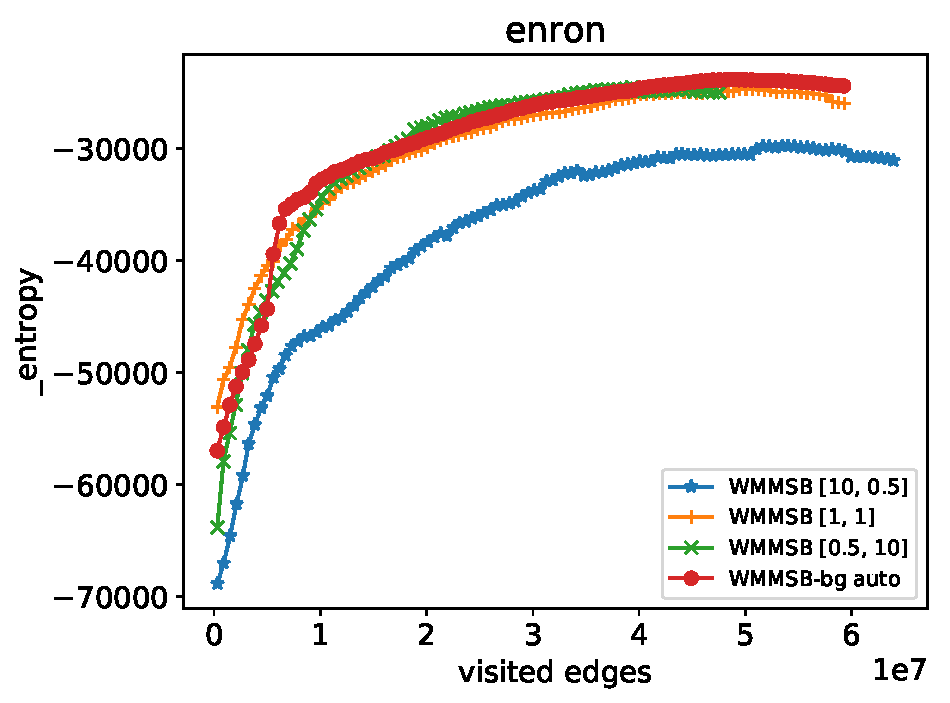
\includegraphics[width=0.32\textwidth]{fig/enron_fig__entropy}
\end{subfigure}
\begin{subfigure}
         \centering
      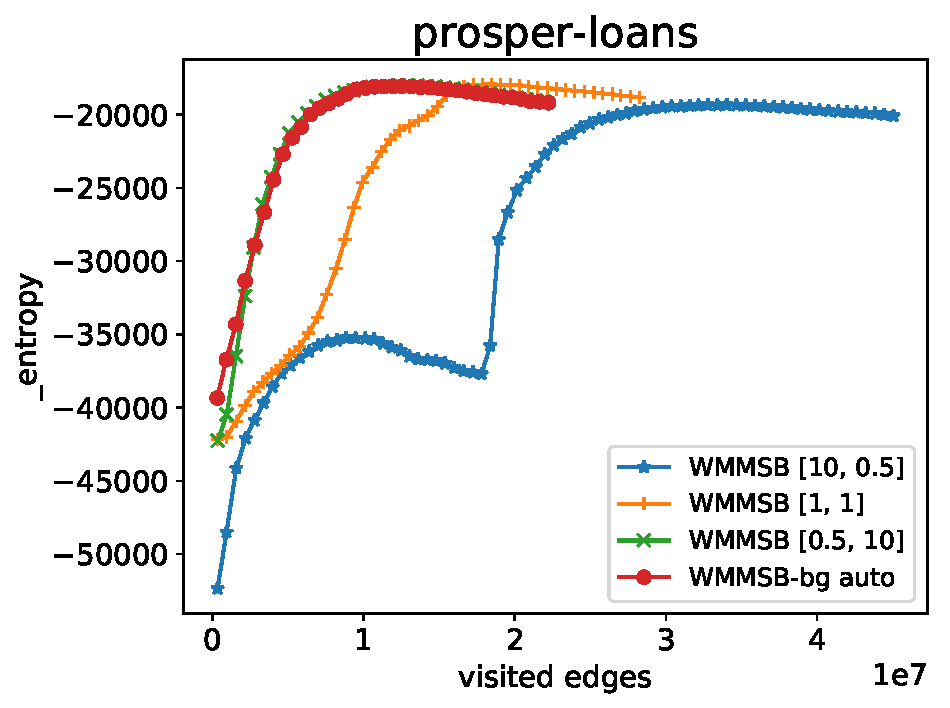
\includegraphics[width=0.32\textwidth]{fig/prosper-loans_fig__entropy}
\end{subfigure}                                                             
\begin{subfigure}                                                           
         \centering                                                         
      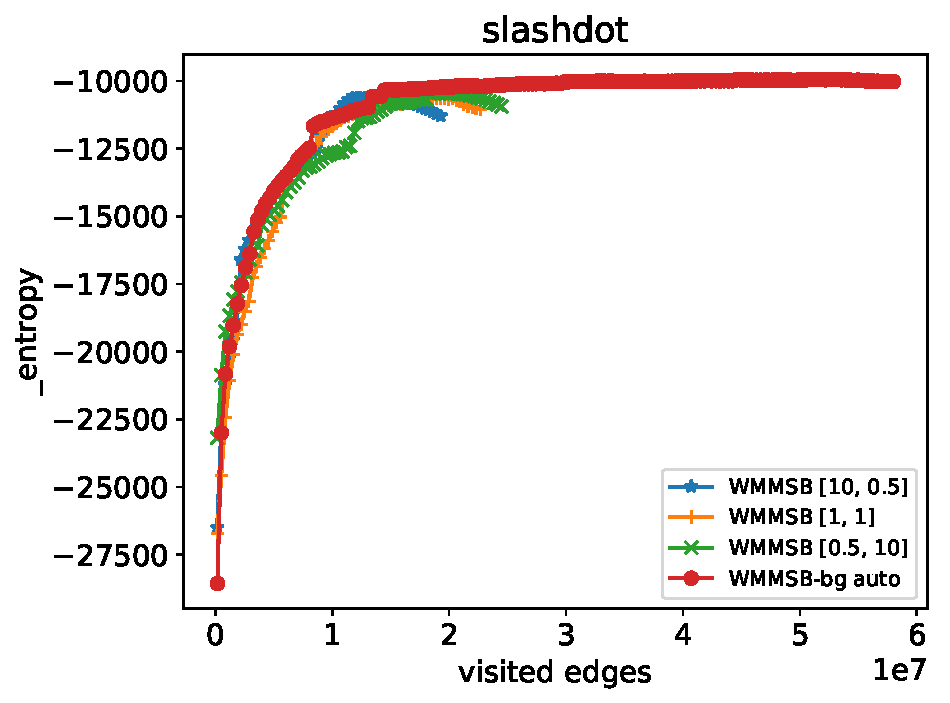
\includegraphics[width=0.32\textwidth]{fig/slashdot_fig__entropy}
\end{subfigure}                                                             
\begin{subfigure}                                                           
         \centering                                                         
      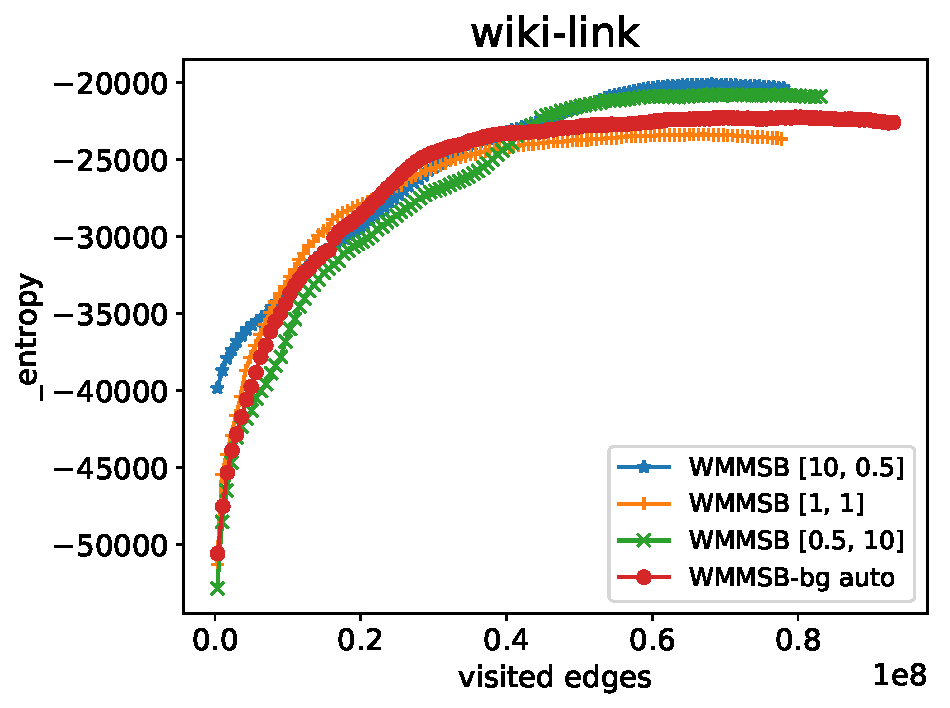
\includegraphics[width=0.32\textwidth]{fig/wiki-link_fig__entropy}
\end{subfigure}                                                             
\begin{subfigure}                                                           
         \centering                                                         
      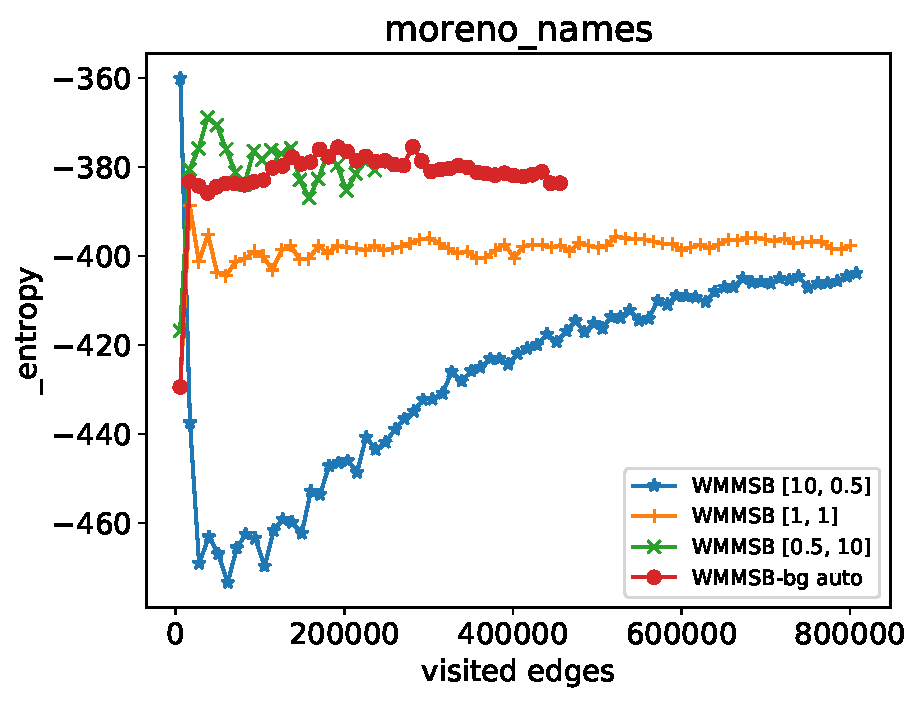
\includegraphics[width=0.32\textwidth]{fig/moreno_names_fig__entropy}
\end{subfigure}                                                             
\caption{Log-likehood convergence for WMMSB and WMMSB-bg models. Three different sets of hyper-parmeter are used for WMMSB.}


    \label{fig:conv_entropy}
\end{figure}

\section{Reproducible Research}

We published our implementation within a platform that aims to ease the development of reproducible complex experiments. We are maintaining this platform that we released under open-source license.\footnote{The name of the project is anonymized.}

To reproduce our results, one can proceed as follows:
\begin{itemize}
\item Install the XXX project:   %\lstinline|git clone https://github.com/*/XXX|  
    \begin{lstlisting}[language=bash]
          $ git clone https://github.com/*/*
          $ cd XXX and make install
    \end{lstlisting}
\item Fit all the models on all the corpus, and save the results:
\begin{lstlisting}[language=bash]
        $ XXX online_roc -x fit -w --repeat 0 1 2 3 4 5 6 7 8 9 
\end{lstlisting}
\item Parallelization can be obtained by adding the options \lstinline|--cores NUMBER_OF_CORES|,
\item Figures can be plotted with the command:  
\begin{lstlisting}[language=bash]
        $ XXX online_roc -x roc_evolution2 --repeat 0 1 2 3 4 5 6 7 8 9
\end{lstlisting}
\end{itemize}



\end{document}

